% Capitolul 15: Recapitulare și pregătire pentru examen
% Serii de timp -- Programele de licență Informatică economică și Cibernetică economică, Academia de Studii Economice din București
% GENERAT de latex/build_chapter15.py -- modificați generatorul, nu acest fișier.

\newcommand{\coursename}{Serii de timp}
\def\tsalang{ro}
% Preambul comun TSA -- Serii de timp / Time Series Analysis (Beamer, 16:9)
% Același design ca MFM și SFM (preluat din SFM, 5 octombrie 2026). Înainte de % Preambul comun TSA -- Serii de timp / Time Series Analysis (Beamer, 16:9)
% Același design ca MFM și SFM (preluat din SFM, 5 octombrie 2026). Înainte de % Preambul comun TSA -- Serii de timp / Time Series Analysis (Beamer, 16:9)
% Același design ca MFM și SFM (preluat din SFM, 5 octombrie 2026). Înainte de \input{../../latex/preamble} se definește
%   \newcommand{\coursename}{Time Series Analysis}      (EN)
%   \newcommand{\coursename}{Serii de timp}       (RO)  și  \def\tsalang{ro}
% Fișierele .tex se află în EN/Courses, EN/Seminars, RO/Cursuri, RO/Seminarii (două niveluri sub rădăcină).
% Deck-urile sînt generate de latex/build_chapterN.py / build_seminarN.py (vezi latex/tsa_build.py).

\documentclass[9pt, aspectratio=169, t]{beamer}
\providecommand{\coursename}{Time Series Analysis}

% Ensure content fits on slides
\setbeamersize{text margin left=8mm, text margin right=8mm}
% Smaller institute font (title page)
\setbeamerfont{institute}{size=\footnotesize}

%=============================================================================
% THEME AND STYLE CONFIGURATION
%=============================================================================
\usetheme{default}
% Using default theme for clean header/footer control

% Color Palette (matching Redispatch PDF)
\definecolor{MainBlue}{RGB}{26, 58, 110}
\definecolor{AccentBlue}{RGB}{26, 58, 110}
\definecolor{IDAred}{RGB}{205, 0, 0}
\definecolor{DarkGray}{RGB}{51, 51, 51}
\definecolor{MediumGray}{RGB}{128, 128, 128}
\definecolor{LightGray}{RGB}{248, 248, 248}
\definecolor{VeryLightGray}{RGB}{235, 235, 235}
\definecolor{KeynoteGray}{RGB}{218, 218, 218}
\definecolor{SectionGray}{RGB}{120, 120, 120}
\definecolor{FooterGray}{RGB}{100, 100, 100}
\definecolor{Crimson}{RGB}{220, 53, 69}
\definecolor{Forest}{RGB}{46, 125, 50}
\definecolor{Amber}{RGB}{181, 133, 63}
\definecolor{Orange}{RGB}{230, 126, 34}
\definecolor{Purple}{RGB}{142, 68, 173}

% Gradient background (exact Keynote 315° gradient: white to RGB 218,218,218)
\setbeamertemplate{background}{%
    \begin{tikzpicture}[remember picture, overlay]
        \shade[shading=axis, shading angle=315,
        top color=white, bottom color=KeynoteGray]
        (current page.south west) rectangle (current page.north east);
    \end{tikzpicture}%
}
% Fallback solid color for compatibility
\setbeamercolor{background canvas}{bg=}

\setbeamercolor{palette primary}{bg=MainBlue, fg=white}
\setbeamercolor{palette secondary}{bg=MainBlue!85, fg=white}
\setbeamercolor{palette tertiary}{bg=MainBlue!70, fg=white}
\setbeamercolor{structure}{fg=MainBlue}
\setbeamercolor{title}{fg=IDAred}
\setbeamercolor{frametitle}{fg=IDAred, bg=}
\setbeamercolor{block title}{bg=MainBlue, fg=white}
\setbeamercolor{block body}{bg=VeryLightGray, fg=DarkGray}
\setbeamercolor{block title alerted}{bg=Crimson, fg=white}
\setbeamercolor{block body alerted}{bg=Crimson!8, fg=DarkGray}
\setbeamercolor{block title example}{bg=Forest, fg=white}
\setbeamercolor{block body example}{bg=Forest!8, fg=DarkGray}
\setbeamercolor{item}{fg=MainBlue}

% Footer colors (override Madrid theme blue)
\setbeamercolor{author in head/foot}{fg=FooterGray, bg=}
\setbeamercolor{title in head/foot}{fg=FooterGray, bg=}
\setbeamercolor{date in head/foot}{fg=FooterGray, bg=}
\setbeamercolor{section in head/foot}{fg=FooterGray, bg=}
\setbeamercolor{subsection in head/foot}{fg=FooterGray, bg=}

% Bullet styles (apply everywhere including blocks)
\setbeamertemplate{itemize item}{\color{MainBlue}$\boxdot$}
\setbeamertemplate{itemize subitem}{\color{MainBlue}$\blacktriangleright$}
\setbeamertemplate{itemize subsubitem}{\color{MainBlue}\tiny$\bullet$}
\setbeamertemplate{itemize/enumerate body begin}{\normalsize}
\setbeamertemplate{itemize/enumerate subbody begin}{\normalsize}

% Item spacing - compact style
\setlength{\leftmargini}{10pt}       % Level 1: minimal indent
\setlength{\leftmarginii}{10pt}      % Level 2: minimal additional indent
% Compact list spacing (zero extra space before/after lists in blocks)
\makeatletter
\def\@listi{\leftmargin\leftmargini \topsep 0pt \parsep 0pt \itemsep 0pt}
\def\@listii{\leftmargin\leftmarginii \topsep 0pt \parsep 0pt \itemsep 0pt}
\makeatother

\setbeamertemplate{navigation symbols}{}

%=============================================================================
% CUSTOM HEADLINE
%=============================================================================
\setbeamertemplate{headline}{%
    \vskip10pt%
    \hbox to \paperwidth{%
        \hskip0.5cm%
        {\small\color{FooterGray}\renewcommand{\hyperlink}[2]{##2}\insertsectionhead}%
        \hfill%
        \textcolor{FooterGray}{\small\insertframenumber}%
        \hskip0.5cm%
    }%
    \vskip4pt%
    {\color{FooterGray}\hrule height 0.4pt}%
}

%=============================================================================
% CUSTOM FOOTER
%=============================================================================
\usepackage{fontawesome5}

\setbeamertemplate{footline}{%
    {\color{FooterGray}\hrule height 0.4pt}%
    \vskip4pt%
    \hbox to \paperwidth{%
        \hskip0.5cm%
        \textcolor{FooterGray}{\small\coursename}%
        \hfill%
        \raisebox{-0.1em}{%
            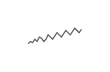
\begin{tikzpicture}[x=0.08em, y=0.08em, line width=0.4pt]
                \draw[FooterGray] (0,3) -- (1,4) -- (2,3.5) -- (3,5) -- (4,4) -- (5,6) -- (6,5.5) -- (7,4) -- (8,5) -- (9,7) -- (10,6) -- (11,5) -- (12,6.5) -- (13,8) -- (14,7) -- (15,6) -- (16,7.5) -- (17,9) -- (18,8) -- (19,7) -- (20,8.5) -- (21,10) -- (22,9) -- (23,8) -- (24,9.5);
            \end{tikzpicture}%
        }%
        \hskip0.5cm%
    }%
    \vskip6pt%
}

%=============================================================================
% PACKAGES
%=============================================================================
\usepackage[utf8]{inputenc}
\DeclareUnicodeCharacter{03B1}{\ensuremath{\alpha}}
\usepackage[T1]{fontenc}
\usepackage{amsmath, amssymb, amsthm}
\usepackage{mathtools}
\usepackage{bm}
\usepackage{tikz}
\usetikzlibrary{arrows.meta, positioning, shapes, calc, decorations.pathreplacing, shadings}
\usepackage{booktabs}
\usepackage{multirow}
\usepackage{array}
\usepackage{graphicx}
\usepackage{animate}
\usepackage{hyperref}
\usepackage{colortbl}
\usepackage{listings}
\lstset{language=Python, basicstyle=\ttfamily\scriptsize, keywordstyle=\color{MainBlue}\bfseries,
  commentstyle=\color{Forest}, stringstyle=\color{Crimson}, breaklines=true,
  frame=none, backgroundcolor=\color{VeryLightGray}, xleftmargin=2mm}
\hypersetup{colorlinks=true, linkcolor=MainBlue, urlcolor=MainBlue}
\graphicspath{{../../logos/}{../../charts/}{../../photos/}}
\usepackage{xcolor}
\hfuzz=2pt  % Suppress tiny overfull warnings (<2pt)
\vfuzz=2pt  % Suppress tiny vertical overfull warnings (<2pt)
% \mathrm in the sans-serif family of the slides (beamer resets \mathrm to the serif family at \begin{document};
% this hook runs after beamer's, so WN, Var, RMSE, ... in formulas match the surrounding text)
% Bold vectors and matrices in the same sans-serif family: \mathbf{A} in sans bold (beamer's own \mathbf came out in
% medium weight), and the bold upright Greek capitals of \boldsymbol / \bm (\bSigma, \bPhi, \boldsymbol{\Theta}) in
% cmss bold: bm.sty fixes its "boldoperators" font when it is loaded (serif cmbx), before beamer switches the
% operators to cmss, so it is reset here.
\AtBeginDocument{%
  \SetMathAlphabet{\mathrm}{normal}{\encodingdefault}{\sfdefault}{\mddefault}{n}%
  \SetMathAlphabet{\mathrm}{bold}{\encodingdefault}{\sfdefault}{bx}{n}%
  \SetMathAlphabet{\mathbf}{normal}{\encodingdefault}{\sfdefault}{bx}{n}%
  \SetMathAlphabet{\mathbf}{bold}{\encodingdefault}{\sfdefault}{bx}{n}%
  \SetSymbolFont{boldoperators}{normal}{OT1}{cmss}{bx}{n}%
  \SetSymbolFont{boldoperators}{bold}{OT1}{cmss}{bx}{n}}

%=============================================================================
% QUANTLET COMMANDS
%   \quantlet{<displayed name>}{<url>}       (generic, compatible with the older TSA decks)
%   \tsaquantlet{Ch_05}{TSA_ch5_garch}       -> https://github.com/danpele/Time-Series-Analysis/tree/main/Quantlets/Ch_05/TSA_ch5_garch
%   \qlurl{<folder>} is defined per chapter by the generator (Quantlets/Ch_NN/<folder>)
%=============================================================================
\newcommand{\tsarepo}{https://github.com/danpele/Time-Series-Analysis}
\newcommand{\tsaqlbase}{https://github.com/danpele/Time-Series-Analysis/tree/main/Quantlets}
\newcommand{\quantlet}[2]{%
    \hfill\href{#2}{%
        \raisebox{-0.15em}{
\includegraphics[height=0.7em]{ql_logo.png}}%
        \textcolor{MainBlue}{\tiny\ #1}%
    }%
}
\newcommand{\tsaquantlet}[2]{\quantlet{\detokenize{#2}}{\tsaqlbase/#1/#2}}

%=============================================================================
% NOTEBOOKS (Google Colab)
%   \colaburl{notebooks/EN/chapter5_seminar_notebook.ipynb} -> the Colab link of a file in the TSA repo
%   \nb: the chapter notebook (each seminar deck redefines it with \renewcommand)
%=============================================================================
\newcommand{\colaburl}[1]{https://colab.research.google.com/github/danpele/Time-Series-Analysis/blob/main/#1}
\newcommand{\nb}{https://colab.research.google.com/github/danpele/Time-Series-Analysis/tree/main/notebooks/EN}
\newcommand{\nbname}{notebooks/EN}

%=============================================================================
% SLIDE HELPERS (used by the generators; the same as in MFM)
%=============================================================================
% local font size for list bodies (the preamble forces \normalsize)
\newcommand{\itemsize}[1]{\setbeamertemplate{itemize/enumerate body begin}{#1}\setbeamertemplate{itemize/enumerate subbody begin}{#1}}
\newcommand{\intitle}[1]{{\hypersetup{urlcolor=white}#1}}   % white links inside coloured title bars
\newcommand{\imgcap}[1]{{\scriptsize #1}\\[0.5mm]}          % caption under a photo
\newcommand{\imgcredit}[2]{{\tiny\color{FooterGray}\href{#1}{#2}}}   % image credit: source URL, author/licence
\newcommand{\aiprompt}[1]{{\ttfamily\color{MainBlue}#1}}     % a prompt to an AI assistant

%=============================================================================
% SEMINARS: student version by default; the instructor wrapper *_solutions.tex sets \solutionstrue
%=============================================================================
\makeatletter\@ifundefined{ifsolutions}{\expandafter\newif\csname ifsolutions\endcsname}{}\makeatother
\newcommand{\solonly}[1]{\ifsolutions #1\fi}
\newcommand{\propsub}{\ifsolutions\else\framesubtitle{\ifdefined\tsalang Rezolvarea se discută la seminar\else Solution discussed in class\fi}\fi}

%=============================================================================
% APPENDIX AND CHAPTER LINKS (latex/appendix_links.py writes the calls; it also re-declares these
% macros before \begin{document}, so the decks compile with or without this preamble block)
%=============================================================================
\providecommand{\tsaapplink}[3]{\hypertarget{#2}{}\hyperlink{#1}{\beamergotobutton{#3}}}
\providecommand{\tsaappback}[2]{\begin{tikzpicture}[remember picture,overlay]\node[anchor=south east] at ([xshift=-3mm,yshift=7mm]current page.south east){\hyperlink{#1}{\beamerreturnbutton{#2}}};\end{tikzpicture}}
\providecommand{\tsachlink}[2]{\href{#1}{#2}}
\providecommand{\tsachlinkt}[2]{\href{#1}{\usebeamercolor[fg]{frametitle}#2}}

%=============================================================================
% QUANTINAR COMMAND: link către un curs Quantinar (subiecte avansate)
%=============================================================================
\newcommand{\quantinar}[2]{%
    \href{#2}{%
        \raisebox{-0.15em}{
\includegraphics[height=0.8em]{qr_logo.png}}%
        \textcolor{MainBlue}{\scriptsize\ #1}%
    }%
}

%=============================================================================
% CUSTOM TITLE PAGE
%=============================================================================
\defbeamertemplate*{title page}{hybrid}[1][]
{
    \vspace{0.2cm}
    % Logos row - top header (with clickable links)
    \begin{center}
        \href{https://www.ase.ro}{
\includegraphics[height=1.0cm]{ase_logo.png}}\hspace{0.3cm}%
        \href{https://theida.net}{
\includegraphics[height=1.0cm]{ida_logo.png}}\hspace{0.3cm}%
        \href{https://blockchain-research-center.com}{
\includegraphics[height=1.0cm]{brc_logo.png}}\hspace{0.3cm}%
        \href{https://www.ai4efin.ase.ro}{
\includegraphics[height=1.0cm]{ai4efin_logo.png}}\hspace{0.3cm}%
        \href{https://ipe.ro/new}{
\includegraphics[height=1.0cm]{acad_logo.png}}\hspace{0.3cm}%
        \href{https://www.digital-finance-msca.com}{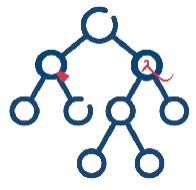
\includegraphics[height=1.0cm]{msca_logo.png}}%
    \end{center}

    \vspace{0.6cm}

    % Main title with Q logos on sides (with clickable links)
    \begin{center}
        \begin{minipage}{0.1\textwidth}
            \centering
            \href{https://quantlet.com}{
\includegraphics[height=1.1cm]{ql_logo.png}}
        \end{minipage}%
        \begin{minipage}{0.78\textwidth}
            \centering
            {\LARGE\bfseries\usebeamercolor[fg]{title}\inserttitle}

            \vspace{0.3cm}

            {\usebeamerfont{subtitle}\usebeamercolor[fg]{title}\insertsubtitle}
        \end{minipage}%
        \begin{minipage}{0.1\textwidth}
            \centering
            \href{https://quantinar.com}{
\includegraphics[height=1.1cm]{qr_logo.png}}
        \end{minipage}
    \end{center}

    \vspace{0.6cm}

    % Authors (left aligned)
    \hspace{0.5cm}{\usebeamerfont{author}\insertauthor}

    \vspace{0.3cm}

    % Institute/Affiliations (left aligned)
    \hspace{0.5cm}\begin{minipage}[t]{0.9\textwidth}
        \raggedright\small\insertinstitute
    \end{minipage}
}

%=============================================================================
% THEOREM ENVIRONMENTS
%=============================================================================
\theoremstyle{definition}
\setbeamertemplate{theorems}[numbered]
\ifdefined\tsalang
\newtheorem{defn}{Definiție}
\newtheorem{thm}{Teoremă}
\newtheorem{prop}{Propoziție}
\newtheorem{rmk}{Observație}
\else
\newtheorem{defn}{Definition}
\newtheorem{thm}{Theorem}
\newtheorem{prop}{Proposition}
\newtheorem{rmk}{Remark}
\fi

%=============================================================================
% CENTRED MINIPAGE (no extra vertical space)
%=============================================================================
\newenvironment{cminipage}[1]{%
    \par\noindent\hfill\begin{minipage}{#1}\ignorespaces
}{%
    \end{minipage}\hfill\null\par
}

%=============================================================================
% CUSTOM COMMANDS
%=============================================================================
\newcommand{\E}{\mathbb{E}}
\newcommand{\Var}{\text{Var}}
\newcommand{\Cov}{\text{Cov}}
\newcommand{\Corr}{\text{Corr}}
\newcommand{\R}{\mathbb{R}}
\newcommand{\N}{\mathbb{N}}
\newcommand{\Z}{\mathbb{Z}}
\newcommand{\B}{\mathbf{B}}
\newcommand{\imark}{\textcolor{MainBlue}{\textbullet}}
\newcommand{\RMSE}{\text{RMSE}}
\newcommand{\MAE}{\text{MAE}}
\newcommand{\MAPE}{\text{MAPE}}

% Boldface vector/matrix commands (VAR, VECM, state space; also used by the older TSA decks)
\newcommand{\bY}{\mathbf{Y}}
\newcommand{\bX}{\mathbf{X}}
\newcommand{\bA}{\mathbf{A}}
\newcommand{\bB}{\mathbf{B}}
\newcommand{\bepsilon}{\boldsymbol{\varepsilon}}
\newcommand{\bSigma}{\boldsymbol{\Sigma}}
\newcommand{\bPhi}{\boldsymbol{\Phi}}
\newcommand{\bGamma}{\boldsymbol{\Gamma}}
\newcommand{\bPi}{\boldsymbol{\Pi}}
\newcommand{\bc}{\mathbf{c}}
\newcommand{\balpha}{\boldsymbol{\alpha}}
\newcommand{\bbeta}{\boldsymbol{\beta}}
\newcommand{\bvarepsilon}{\boldsymbol{\varepsilon}}

% Legacy seminar marks (older TSA seminar decks)
\newcommand{\correct}{\textcolor{Forest}{\checkmark}}
\newcommand{\incorrect}{\textcolor{Crimson}{\texttimes}}
 se definește
%   \newcommand{\coursename}{Time Series Analysis}      (EN)
%   \newcommand{\coursename}{Serii de timp}       (RO)  și  \def\tsalang{ro}
% Fișierele .tex se află în EN/Courses, EN/Seminars, RO/Cursuri, RO/Seminarii (două niveluri sub rădăcină).
% Deck-urile sînt generate de latex/build_chapterN.py / build_seminarN.py (vezi latex/tsa_build.py).

\documentclass[9pt, aspectratio=169, t]{beamer}
\providecommand{\coursename}{Time Series Analysis}

% Ensure content fits on slides
\setbeamersize{text margin left=8mm, text margin right=8mm}
% Smaller institute font (title page)
\setbeamerfont{institute}{size=\footnotesize}

%=============================================================================
% THEME AND STYLE CONFIGURATION
%=============================================================================
\usetheme{default}
% Using default theme for clean header/footer control

% Color Palette (matching Redispatch PDF)
\definecolor{MainBlue}{RGB}{26, 58, 110}
\definecolor{AccentBlue}{RGB}{26, 58, 110}
\definecolor{IDAred}{RGB}{205, 0, 0}
\definecolor{DarkGray}{RGB}{51, 51, 51}
\definecolor{MediumGray}{RGB}{128, 128, 128}
\definecolor{LightGray}{RGB}{248, 248, 248}
\definecolor{VeryLightGray}{RGB}{235, 235, 235}
\definecolor{KeynoteGray}{RGB}{218, 218, 218}
\definecolor{SectionGray}{RGB}{120, 120, 120}
\definecolor{FooterGray}{RGB}{100, 100, 100}
\definecolor{Crimson}{RGB}{220, 53, 69}
\definecolor{Forest}{RGB}{46, 125, 50}
\definecolor{Amber}{RGB}{181, 133, 63}
\definecolor{Orange}{RGB}{230, 126, 34}
\definecolor{Purple}{RGB}{142, 68, 173}

% Gradient background (exact Keynote 315° gradient: white to RGB 218,218,218)
\setbeamertemplate{background}{%
    \begin{tikzpicture}[remember picture, overlay]
        \shade[shading=axis, shading angle=315,
        top color=white, bottom color=KeynoteGray]
        (current page.south west) rectangle (current page.north east);
    \end{tikzpicture}%
}
% Fallback solid color for compatibility
\setbeamercolor{background canvas}{bg=}

\setbeamercolor{palette primary}{bg=MainBlue, fg=white}
\setbeamercolor{palette secondary}{bg=MainBlue!85, fg=white}
\setbeamercolor{palette tertiary}{bg=MainBlue!70, fg=white}
\setbeamercolor{structure}{fg=MainBlue}
\setbeamercolor{title}{fg=IDAred}
\setbeamercolor{frametitle}{fg=IDAred, bg=}
\setbeamercolor{block title}{bg=MainBlue, fg=white}
\setbeamercolor{block body}{bg=VeryLightGray, fg=DarkGray}
\setbeamercolor{block title alerted}{bg=Crimson, fg=white}
\setbeamercolor{block body alerted}{bg=Crimson!8, fg=DarkGray}
\setbeamercolor{block title example}{bg=Forest, fg=white}
\setbeamercolor{block body example}{bg=Forest!8, fg=DarkGray}
\setbeamercolor{item}{fg=MainBlue}

% Footer colors (override Madrid theme blue)
\setbeamercolor{author in head/foot}{fg=FooterGray, bg=}
\setbeamercolor{title in head/foot}{fg=FooterGray, bg=}
\setbeamercolor{date in head/foot}{fg=FooterGray, bg=}
\setbeamercolor{section in head/foot}{fg=FooterGray, bg=}
\setbeamercolor{subsection in head/foot}{fg=FooterGray, bg=}

% Bullet styles (apply everywhere including blocks)
\setbeamertemplate{itemize item}{\color{MainBlue}$\boxdot$}
\setbeamertemplate{itemize subitem}{\color{MainBlue}$\blacktriangleright$}
\setbeamertemplate{itemize subsubitem}{\color{MainBlue}\tiny$\bullet$}
\setbeamertemplate{itemize/enumerate body begin}{\normalsize}
\setbeamertemplate{itemize/enumerate subbody begin}{\normalsize}

% Item spacing - compact style
\setlength{\leftmargini}{10pt}       % Level 1: minimal indent
\setlength{\leftmarginii}{10pt}      % Level 2: minimal additional indent
% Compact list spacing (zero extra space before/after lists in blocks)
\makeatletter
\def\@listi{\leftmargin\leftmargini \topsep 0pt \parsep 0pt \itemsep 0pt}
\def\@listii{\leftmargin\leftmarginii \topsep 0pt \parsep 0pt \itemsep 0pt}
\makeatother

\setbeamertemplate{navigation symbols}{}

%=============================================================================
% CUSTOM HEADLINE
%=============================================================================
\setbeamertemplate{headline}{%
    \vskip10pt%
    \hbox to \paperwidth{%
        \hskip0.5cm%
        {\small\color{FooterGray}\renewcommand{\hyperlink}[2]{##2}\insertsectionhead}%
        \hfill%
        \textcolor{FooterGray}{\small\insertframenumber}%
        \hskip0.5cm%
    }%
    \vskip4pt%
    {\color{FooterGray}\hrule height 0.4pt}%
}

%=============================================================================
% CUSTOM FOOTER
%=============================================================================
\usepackage{fontawesome5}

\setbeamertemplate{footline}{%
    {\color{FooterGray}\hrule height 0.4pt}%
    \vskip4pt%
    \hbox to \paperwidth{%
        \hskip0.5cm%
        \textcolor{FooterGray}{\small\coursename}%
        \hfill%
        \raisebox{-0.1em}{%
            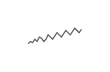
\begin{tikzpicture}[x=0.08em, y=0.08em, line width=0.4pt]
                \draw[FooterGray] (0,3) -- (1,4) -- (2,3.5) -- (3,5) -- (4,4) -- (5,6) -- (6,5.5) -- (7,4) -- (8,5) -- (9,7) -- (10,6) -- (11,5) -- (12,6.5) -- (13,8) -- (14,7) -- (15,6) -- (16,7.5) -- (17,9) -- (18,8) -- (19,7) -- (20,8.5) -- (21,10) -- (22,9) -- (23,8) -- (24,9.5);
            \end{tikzpicture}%
        }%
        \hskip0.5cm%
    }%
    \vskip6pt%
}

%=============================================================================
% PACKAGES
%=============================================================================
\usepackage[utf8]{inputenc}
\DeclareUnicodeCharacter{03B1}{\ensuremath{\alpha}}
\usepackage[T1]{fontenc}
\usepackage{amsmath, amssymb, amsthm}
\usepackage{mathtools}
\usepackage{bm}
\usepackage{tikz}
\usetikzlibrary{arrows.meta, positioning, shapes, calc, decorations.pathreplacing, shadings}
\usepackage{booktabs}
\usepackage{multirow}
\usepackage{array}
\usepackage{graphicx}
\usepackage{animate}
\usepackage{hyperref}
\usepackage{colortbl}
\usepackage{listings}
\lstset{language=Python, basicstyle=\ttfamily\scriptsize, keywordstyle=\color{MainBlue}\bfseries,
  commentstyle=\color{Forest}, stringstyle=\color{Crimson}, breaklines=true,
  frame=none, backgroundcolor=\color{VeryLightGray}, xleftmargin=2mm}
\hypersetup{colorlinks=true, linkcolor=MainBlue, urlcolor=MainBlue}
\graphicspath{{../../logos/}{../../charts/}{../../photos/}}
\usepackage{xcolor}
\hfuzz=2pt  % Suppress tiny overfull warnings (<2pt)
\vfuzz=2pt  % Suppress tiny vertical overfull warnings (<2pt)
% \mathrm in the sans-serif family of the slides (beamer resets \mathrm to the serif family at \begin{document};
% this hook runs after beamer's, so WN, Var, RMSE, ... in formulas match the surrounding text)
% Bold vectors and matrices in the same sans-serif family: \mathbf{A} in sans bold (beamer's own \mathbf came out in
% medium weight), and the bold upright Greek capitals of \boldsymbol / \bm (\bSigma, \bPhi, \boldsymbol{\Theta}) in
% cmss bold: bm.sty fixes its "boldoperators" font when it is loaded (serif cmbx), before beamer switches the
% operators to cmss, so it is reset here.
\AtBeginDocument{%
  \SetMathAlphabet{\mathrm}{normal}{\encodingdefault}{\sfdefault}{\mddefault}{n}%
  \SetMathAlphabet{\mathrm}{bold}{\encodingdefault}{\sfdefault}{bx}{n}%
  \SetMathAlphabet{\mathbf}{normal}{\encodingdefault}{\sfdefault}{bx}{n}%
  \SetMathAlphabet{\mathbf}{bold}{\encodingdefault}{\sfdefault}{bx}{n}%
  \SetSymbolFont{boldoperators}{normal}{OT1}{cmss}{bx}{n}%
  \SetSymbolFont{boldoperators}{bold}{OT1}{cmss}{bx}{n}}

%=============================================================================
% QUANTLET COMMANDS
%   \quantlet{<displayed name>}{<url>}       (generic, compatible with the older TSA decks)
%   \tsaquantlet{Ch_05}{TSA_ch5_garch}       -> https://github.com/danpele/Time-Series-Analysis/tree/main/Quantlets/Ch_05/TSA_ch5_garch
%   \qlurl{<folder>} is defined per chapter by the generator (Quantlets/Ch_NN/<folder>)
%=============================================================================
\newcommand{\tsarepo}{https://github.com/danpele/Time-Series-Analysis}
\newcommand{\tsaqlbase}{https://github.com/danpele/Time-Series-Analysis/tree/main/Quantlets}
\newcommand{\quantlet}[2]{%
    \hfill\href{#2}{%
        \raisebox{-0.15em}{
\includegraphics[height=0.7em]{ql_logo.png}}%
        \textcolor{MainBlue}{\tiny\ #1}%
    }%
}
\newcommand{\tsaquantlet}[2]{\quantlet{\detokenize{#2}}{\tsaqlbase/#1/#2}}

%=============================================================================
% NOTEBOOKS (Google Colab)
%   \colaburl{notebooks/EN/chapter5_seminar_notebook.ipynb} -> the Colab link of a file in the TSA repo
%   \nb: the chapter notebook (each seminar deck redefines it with \renewcommand)
%=============================================================================
\newcommand{\colaburl}[1]{https://colab.research.google.com/github/danpele/Time-Series-Analysis/blob/main/#1}
\newcommand{\nb}{https://colab.research.google.com/github/danpele/Time-Series-Analysis/tree/main/notebooks/EN}
\newcommand{\nbname}{notebooks/EN}

%=============================================================================
% SLIDE HELPERS (used by the generators; the same as in MFM)
%=============================================================================
% local font size for list bodies (the preamble forces \normalsize)
\newcommand{\itemsize}[1]{\setbeamertemplate{itemize/enumerate body begin}{#1}\setbeamertemplate{itemize/enumerate subbody begin}{#1}}
\newcommand{\intitle}[1]{{\hypersetup{urlcolor=white}#1}}   % white links inside coloured title bars
\newcommand{\imgcap}[1]{{\scriptsize #1}\\[0.5mm]}          % caption under a photo
\newcommand{\imgcredit}[2]{{\tiny\color{FooterGray}\href{#1}{#2}}}   % image credit: source URL, author/licence
\newcommand{\aiprompt}[1]{{\ttfamily\color{MainBlue}#1}}     % a prompt to an AI assistant

%=============================================================================
% SEMINARS: student version by default; the instructor wrapper *_solutions.tex sets \solutionstrue
%=============================================================================
\makeatletter\@ifundefined{ifsolutions}{\expandafter\newif\csname ifsolutions\endcsname}{}\makeatother
\newcommand{\solonly}[1]{\ifsolutions #1\fi}
\newcommand{\propsub}{\ifsolutions\else\framesubtitle{\ifdefined\tsalang Rezolvarea se discută la seminar\else Solution discussed in class\fi}\fi}

%=============================================================================
% APPENDIX AND CHAPTER LINKS (latex/appendix_links.py writes the calls; it also re-declares these
% macros before \begin{document}, so the decks compile with or without this preamble block)
%=============================================================================
\providecommand{\tsaapplink}[3]{\hypertarget{#2}{}\hyperlink{#1}{\beamergotobutton{#3}}}
\providecommand{\tsaappback}[2]{\begin{tikzpicture}[remember picture,overlay]\node[anchor=south east] at ([xshift=-3mm,yshift=7mm]current page.south east){\hyperlink{#1}{\beamerreturnbutton{#2}}};\end{tikzpicture}}
\providecommand{\tsachlink}[2]{\href{#1}{#2}}
\providecommand{\tsachlinkt}[2]{\href{#1}{\usebeamercolor[fg]{frametitle}#2}}

%=============================================================================
% QUANTINAR COMMAND: link către un curs Quantinar (subiecte avansate)
%=============================================================================
\newcommand{\quantinar}[2]{%
    \href{#2}{%
        \raisebox{-0.15em}{
\includegraphics[height=0.8em]{qr_logo.png}}%
        \textcolor{MainBlue}{\scriptsize\ #1}%
    }%
}

%=============================================================================
% CUSTOM TITLE PAGE
%=============================================================================
\defbeamertemplate*{title page}{hybrid}[1][]
{
    \vspace{0.2cm}
    % Logos row - top header (with clickable links)
    \begin{center}
        \href{https://www.ase.ro}{
\includegraphics[height=1.0cm]{ase_logo.png}}\hspace{0.3cm}%
        \href{https://theida.net}{
\includegraphics[height=1.0cm]{ida_logo.png}}\hspace{0.3cm}%
        \href{https://blockchain-research-center.com}{
\includegraphics[height=1.0cm]{brc_logo.png}}\hspace{0.3cm}%
        \href{https://www.ai4efin.ase.ro}{
\includegraphics[height=1.0cm]{ai4efin_logo.png}}\hspace{0.3cm}%
        \href{https://ipe.ro/new}{
\includegraphics[height=1.0cm]{acad_logo.png}}\hspace{0.3cm}%
        \href{https://www.digital-finance-msca.com}{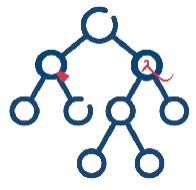
\includegraphics[height=1.0cm]{msca_logo.png}}%
    \end{center}

    \vspace{0.6cm}

    % Main title with Q logos on sides (with clickable links)
    \begin{center}
        \begin{minipage}{0.1\textwidth}
            \centering
            \href{https://quantlet.com}{
\includegraphics[height=1.1cm]{ql_logo.png}}
        \end{minipage}%
        \begin{minipage}{0.78\textwidth}
            \centering
            {\LARGE\bfseries\usebeamercolor[fg]{title}\inserttitle}

            \vspace{0.3cm}

            {\usebeamerfont{subtitle}\usebeamercolor[fg]{title}\insertsubtitle}
        \end{minipage}%
        \begin{minipage}{0.1\textwidth}
            \centering
            \href{https://quantinar.com}{
\includegraphics[height=1.1cm]{qr_logo.png}}
        \end{minipage}
    \end{center}

    \vspace{0.6cm}

    % Authors (left aligned)
    \hspace{0.5cm}{\usebeamerfont{author}\insertauthor}

    \vspace{0.3cm}

    % Institute/Affiliations (left aligned)
    \hspace{0.5cm}\begin{minipage}[t]{0.9\textwidth}
        \raggedright\small\insertinstitute
    \end{minipage}
}

%=============================================================================
% THEOREM ENVIRONMENTS
%=============================================================================
\theoremstyle{definition}
\setbeamertemplate{theorems}[numbered]
\ifdefined\tsalang
\newtheorem{defn}{Definiție}
\newtheorem{thm}{Teoremă}
\newtheorem{prop}{Propoziție}
\newtheorem{rmk}{Observație}
\else
\newtheorem{defn}{Definition}
\newtheorem{thm}{Theorem}
\newtheorem{prop}{Proposition}
\newtheorem{rmk}{Remark}
\fi

%=============================================================================
% CENTRED MINIPAGE (no extra vertical space)
%=============================================================================
\newenvironment{cminipage}[1]{%
    \par\noindent\hfill\begin{minipage}{#1}\ignorespaces
}{%
    \end{minipage}\hfill\null\par
}

%=============================================================================
% CUSTOM COMMANDS
%=============================================================================
\newcommand{\E}{\mathbb{E}}
\newcommand{\Var}{\text{Var}}
\newcommand{\Cov}{\text{Cov}}
\newcommand{\Corr}{\text{Corr}}
\newcommand{\R}{\mathbb{R}}
\newcommand{\N}{\mathbb{N}}
\newcommand{\Z}{\mathbb{Z}}
\newcommand{\B}{\mathbf{B}}
\newcommand{\imark}{\textcolor{MainBlue}{\textbullet}}
\newcommand{\RMSE}{\text{RMSE}}
\newcommand{\MAE}{\text{MAE}}
\newcommand{\MAPE}{\text{MAPE}}

% Boldface vector/matrix commands (VAR, VECM, state space; also used by the older TSA decks)
\newcommand{\bY}{\mathbf{Y}}
\newcommand{\bX}{\mathbf{X}}
\newcommand{\bA}{\mathbf{A}}
\newcommand{\bB}{\mathbf{B}}
\newcommand{\bepsilon}{\boldsymbol{\varepsilon}}
\newcommand{\bSigma}{\boldsymbol{\Sigma}}
\newcommand{\bPhi}{\boldsymbol{\Phi}}
\newcommand{\bGamma}{\boldsymbol{\Gamma}}
\newcommand{\bPi}{\boldsymbol{\Pi}}
\newcommand{\bc}{\mathbf{c}}
\newcommand{\balpha}{\boldsymbol{\alpha}}
\newcommand{\bbeta}{\boldsymbol{\beta}}
\newcommand{\bvarepsilon}{\boldsymbol{\varepsilon}}

% Legacy seminar marks (older TSA seminar decks)
\newcommand{\correct}{\textcolor{Forest}{\checkmark}}
\newcommand{\incorrect}{\textcolor{Crimson}{\texttimes}}
 se definește
%   \newcommand{\coursename}{Time Series Analysis}      (EN)
%   \newcommand{\coursename}{Serii de timp}       (RO)  și  \def\tsalang{ro}
% Fișierele .tex se află în EN/Courses, EN/Seminars, RO/Cursuri, RO/Seminarii (două niveluri sub rădăcină).
% Deck-urile sînt generate de latex/build_chapterN.py / build_seminarN.py (vezi latex/tsa_build.py).

\documentclass[9pt, aspectratio=169, t]{beamer}
\providecommand{\coursename}{Time Series Analysis}

% Ensure content fits on slides
\setbeamersize{text margin left=8mm, text margin right=8mm}
% Smaller institute font (title page)
\setbeamerfont{institute}{size=\footnotesize}

%=============================================================================
% THEME AND STYLE CONFIGURATION
%=============================================================================
\usetheme{default}
% Using default theme for clean header/footer control

% Color Palette (matching Redispatch PDF)
\definecolor{MainBlue}{RGB}{26, 58, 110}
\definecolor{AccentBlue}{RGB}{26, 58, 110}
\definecolor{IDAred}{RGB}{205, 0, 0}
\definecolor{DarkGray}{RGB}{51, 51, 51}
\definecolor{MediumGray}{RGB}{128, 128, 128}
\definecolor{LightGray}{RGB}{248, 248, 248}
\definecolor{VeryLightGray}{RGB}{235, 235, 235}
\definecolor{KeynoteGray}{RGB}{218, 218, 218}
\definecolor{SectionGray}{RGB}{120, 120, 120}
\definecolor{FooterGray}{RGB}{100, 100, 100}
\definecolor{Crimson}{RGB}{220, 53, 69}
\definecolor{Forest}{RGB}{46, 125, 50}
\definecolor{Amber}{RGB}{181, 133, 63}
\definecolor{Orange}{RGB}{230, 126, 34}
\definecolor{Purple}{RGB}{142, 68, 173}

% Gradient background (exact Keynote 315° gradient: white to RGB 218,218,218)
\setbeamertemplate{background}{%
    \begin{tikzpicture}[remember picture, overlay]
        \shade[shading=axis, shading angle=315,
        top color=white, bottom color=KeynoteGray]
        (current page.south west) rectangle (current page.north east);
    \end{tikzpicture}%
}
% Fallback solid color for compatibility
\setbeamercolor{background canvas}{bg=}

\setbeamercolor{palette primary}{bg=MainBlue, fg=white}
\setbeamercolor{palette secondary}{bg=MainBlue!85, fg=white}
\setbeamercolor{palette tertiary}{bg=MainBlue!70, fg=white}
\setbeamercolor{structure}{fg=MainBlue}
\setbeamercolor{title}{fg=IDAred}
\setbeamercolor{frametitle}{fg=IDAred, bg=}
\setbeamercolor{block title}{bg=MainBlue, fg=white}
\setbeamercolor{block body}{bg=VeryLightGray, fg=DarkGray}
\setbeamercolor{block title alerted}{bg=Crimson, fg=white}
\setbeamercolor{block body alerted}{bg=Crimson!8, fg=DarkGray}
\setbeamercolor{block title example}{bg=Forest, fg=white}
\setbeamercolor{block body example}{bg=Forest!8, fg=DarkGray}
\setbeamercolor{item}{fg=MainBlue}

% Footer colors (override Madrid theme blue)
\setbeamercolor{author in head/foot}{fg=FooterGray, bg=}
\setbeamercolor{title in head/foot}{fg=FooterGray, bg=}
\setbeamercolor{date in head/foot}{fg=FooterGray, bg=}
\setbeamercolor{section in head/foot}{fg=FooterGray, bg=}
\setbeamercolor{subsection in head/foot}{fg=FooterGray, bg=}

% Bullet styles (apply everywhere including blocks)
\setbeamertemplate{itemize item}{\color{MainBlue}$\boxdot$}
\setbeamertemplate{itemize subitem}{\color{MainBlue}$\blacktriangleright$}
\setbeamertemplate{itemize subsubitem}{\color{MainBlue}\tiny$\bullet$}
\setbeamertemplate{itemize/enumerate body begin}{\normalsize}
\setbeamertemplate{itemize/enumerate subbody begin}{\normalsize}

% Item spacing - compact style
\setlength{\leftmargini}{10pt}       % Level 1: minimal indent
\setlength{\leftmarginii}{10pt}      % Level 2: minimal additional indent
% Compact list spacing (zero extra space before/after lists in blocks)
\makeatletter
\def\@listi{\leftmargin\leftmargini \topsep 0pt \parsep 0pt \itemsep 0pt}
\def\@listii{\leftmargin\leftmarginii \topsep 0pt \parsep 0pt \itemsep 0pt}
\makeatother

\setbeamertemplate{navigation symbols}{}

%=============================================================================
% CUSTOM HEADLINE
%=============================================================================
\setbeamertemplate{headline}{%
    \vskip10pt%
    \hbox to \paperwidth{%
        \hskip0.5cm%
        {\small\color{FooterGray}\renewcommand{\hyperlink}[2]{##2}\insertsectionhead}%
        \hfill%
        \textcolor{FooterGray}{\small\insertframenumber}%
        \hskip0.5cm%
    }%
    \vskip4pt%
    {\color{FooterGray}\hrule height 0.4pt}%
}

%=============================================================================
% CUSTOM FOOTER
%=============================================================================
\usepackage{fontawesome5}

\setbeamertemplate{footline}{%
    {\color{FooterGray}\hrule height 0.4pt}%
    \vskip4pt%
    \hbox to \paperwidth{%
        \hskip0.5cm%
        \textcolor{FooterGray}{\small\coursename}%
        \hfill%
        \raisebox{-0.1em}{%
            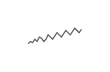
\begin{tikzpicture}[x=0.08em, y=0.08em, line width=0.4pt]
                \draw[FooterGray] (0,3) -- (1,4) -- (2,3.5) -- (3,5) -- (4,4) -- (5,6) -- (6,5.5) -- (7,4) -- (8,5) -- (9,7) -- (10,6) -- (11,5) -- (12,6.5) -- (13,8) -- (14,7) -- (15,6) -- (16,7.5) -- (17,9) -- (18,8) -- (19,7) -- (20,8.5) -- (21,10) -- (22,9) -- (23,8) -- (24,9.5);
            \end{tikzpicture}%
        }%
        \hskip0.5cm%
    }%
    \vskip6pt%
}

%=============================================================================
% PACKAGES
%=============================================================================
\usepackage[utf8]{inputenc}
\DeclareUnicodeCharacter{03B1}{\ensuremath{\alpha}}
\usepackage[T1]{fontenc}
\usepackage{amsmath, amssymb, amsthm}
\usepackage{mathtools}
\usepackage{bm}
\usepackage{tikz}
\usetikzlibrary{arrows.meta, positioning, shapes, calc, decorations.pathreplacing, shadings}
\usepackage{booktabs}
\usepackage{multirow}
\usepackage{array}
\usepackage{graphicx}
\usepackage{animate}
\usepackage{hyperref}
\usepackage{colortbl}
\usepackage{listings}
\lstset{language=Python, basicstyle=\ttfamily\scriptsize, keywordstyle=\color{MainBlue}\bfseries,
  commentstyle=\color{Forest}, stringstyle=\color{Crimson}, breaklines=true,
  frame=none, backgroundcolor=\color{VeryLightGray}, xleftmargin=2mm}
\hypersetup{colorlinks=true, linkcolor=MainBlue, urlcolor=MainBlue}
\graphicspath{{../../logos/}{../../charts/}{../../photos/}}
\usepackage{xcolor}
\hfuzz=2pt  % Suppress tiny overfull warnings (<2pt)
\vfuzz=2pt  % Suppress tiny vertical overfull warnings (<2pt)
% \mathrm in the sans-serif family of the slides (beamer resets \mathrm to the serif family at \begin{document};
% this hook runs after beamer's, so WN, Var, RMSE, ... in formulas match the surrounding text)
% Bold vectors and matrices in the same sans-serif family: \mathbf{A} in sans bold (beamer's own \mathbf came out in
% medium weight), and the bold upright Greek capitals of \boldsymbol / \bm (\bSigma, \bPhi, \boldsymbol{\Theta}) in
% cmss bold: bm.sty fixes its "boldoperators" font when it is loaded (serif cmbx), before beamer switches the
% operators to cmss, so it is reset here.
\AtBeginDocument{%
  \SetMathAlphabet{\mathrm}{normal}{\encodingdefault}{\sfdefault}{\mddefault}{n}%
  \SetMathAlphabet{\mathrm}{bold}{\encodingdefault}{\sfdefault}{bx}{n}%
  \SetMathAlphabet{\mathbf}{normal}{\encodingdefault}{\sfdefault}{bx}{n}%
  \SetMathAlphabet{\mathbf}{bold}{\encodingdefault}{\sfdefault}{bx}{n}%
  \SetSymbolFont{boldoperators}{normal}{OT1}{cmss}{bx}{n}%
  \SetSymbolFont{boldoperators}{bold}{OT1}{cmss}{bx}{n}}

%=============================================================================
% QUANTLET COMMANDS
%   \quantlet{<displayed name>}{<url>}       (generic, compatible with the older TSA decks)
%   \tsaquantlet{Ch_05}{TSA_ch5_garch}       -> https://github.com/danpele/Time-Series-Analysis/tree/main/Quantlets/Ch_05/TSA_ch5_garch
%   \qlurl{<folder>} is defined per chapter by the generator (Quantlets/Ch_NN/<folder>)
%=============================================================================
\newcommand{\tsarepo}{https://github.com/danpele/Time-Series-Analysis}
\newcommand{\tsaqlbase}{https://github.com/danpele/Time-Series-Analysis/tree/main/Quantlets}
\newcommand{\quantlet}[2]{%
    \hfill\href{#2}{%
        \raisebox{-0.15em}{
\includegraphics[height=0.7em]{ql_logo.png}}%
        \textcolor{MainBlue}{\tiny\ #1}%
    }%
}
\newcommand{\tsaquantlet}[2]{\quantlet{\detokenize{#2}}{\tsaqlbase/#1/#2}}

%=============================================================================
% NOTEBOOKS (Google Colab)
%   \colaburl{notebooks/EN/chapter5_seminar_notebook.ipynb} -> the Colab link of a file in the TSA repo
%   \nb: the chapter notebook (each seminar deck redefines it with \renewcommand)
%=============================================================================
\newcommand{\colaburl}[1]{https://colab.research.google.com/github/danpele/Time-Series-Analysis/blob/main/#1}
\newcommand{\nb}{https://colab.research.google.com/github/danpele/Time-Series-Analysis/tree/main/notebooks/EN}
\newcommand{\nbname}{notebooks/EN}

%=============================================================================
% SLIDE HELPERS (used by the generators; the same as in MFM)
%=============================================================================
% local font size for list bodies (the preamble forces \normalsize)
\newcommand{\itemsize}[1]{\setbeamertemplate{itemize/enumerate body begin}{#1}\setbeamertemplate{itemize/enumerate subbody begin}{#1}}
\newcommand{\intitle}[1]{{\hypersetup{urlcolor=white}#1}}   % white links inside coloured title bars
\newcommand{\imgcap}[1]{{\scriptsize #1}\\[0.5mm]}          % caption under a photo
\newcommand{\imgcredit}[2]{{\tiny\color{FooterGray}\href{#1}{#2}}}   % image credit: source URL, author/licence
\newcommand{\aiprompt}[1]{{\ttfamily\color{MainBlue}#1}}     % a prompt to an AI assistant

%=============================================================================
% SEMINARS: student version by default; the instructor wrapper *_solutions.tex sets \solutionstrue
%=============================================================================
\makeatletter\@ifundefined{ifsolutions}{\expandafter\newif\csname ifsolutions\endcsname}{}\makeatother
\newcommand{\solonly}[1]{\ifsolutions #1\fi}
\newcommand{\propsub}{\ifsolutions\else\framesubtitle{\ifdefined\tsalang Rezolvarea se discută la seminar\else Solution discussed in class\fi}\fi}

%=============================================================================
% APPENDIX AND CHAPTER LINKS (latex/appendix_links.py writes the calls; it also re-declares these
% macros before \begin{document}, so the decks compile with or without this preamble block)
%=============================================================================
\providecommand{\tsaapplink}[3]{\hypertarget{#2}{}\hyperlink{#1}{\beamergotobutton{#3}}}
\providecommand{\tsaappback}[2]{\begin{tikzpicture}[remember picture,overlay]\node[anchor=south east] at ([xshift=-3mm,yshift=7mm]current page.south east){\hyperlink{#1}{\beamerreturnbutton{#2}}};\end{tikzpicture}}
\providecommand{\tsachlink}[2]{\href{#1}{#2}}
\providecommand{\tsachlinkt}[2]{\href{#1}{\usebeamercolor[fg]{frametitle}#2}}

%=============================================================================
% QUANTINAR COMMAND: link către un curs Quantinar (subiecte avansate)
%=============================================================================
\newcommand{\quantinar}[2]{%
    \href{#2}{%
        \raisebox{-0.15em}{
\includegraphics[height=0.8em]{qr_logo.png}}%
        \textcolor{MainBlue}{\scriptsize\ #1}%
    }%
}

%=============================================================================
% CUSTOM TITLE PAGE
%=============================================================================
\defbeamertemplate*{title page}{hybrid}[1][]
{
    \vspace{0.2cm}
    % Logos row - top header (with clickable links)
    \begin{center}
        \href{https://www.ase.ro}{
\includegraphics[height=1.0cm]{ase_logo.png}}\hspace{0.3cm}%
        \href{https://theida.net}{
\includegraphics[height=1.0cm]{ida_logo.png}}\hspace{0.3cm}%
        \href{https://blockchain-research-center.com}{
\includegraphics[height=1.0cm]{brc_logo.png}}\hspace{0.3cm}%
        \href{https://www.ai4efin.ase.ro}{
\includegraphics[height=1.0cm]{ai4efin_logo.png}}\hspace{0.3cm}%
        \href{https://ipe.ro/new}{
\includegraphics[height=1.0cm]{acad_logo.png}}\hspace{0.3cm}%
        \href{https://www.digital-finance-msca.com}{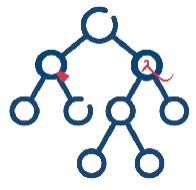
\includegraphics[height=1.0cm]{msca_logo.png}}%
    \end{center}

    \vspace{0.6cm}

    % Main title with Q logos on sides (with clickable links)
    \begin{center}
        \begin{minipage}{0.1\textwidth}
            \centering
            \href{https://quantlet.com}{
\includegraphics[height=1.1cm]{ql_logo.png}}
        \end{minipage}%
        \begin{minipage}{0.78\textwidth}
            \centering
            {\LARGE\bfseries\usebeamercolor[fg]{title}\inserttitle}

            \vspace{0.3cm}

            {\usebeamerfont{subtitle}\usebeamercolor[fg]{title}\insertsubtitle}
        \end{minipage}%
        \begin{minipage}{0.1\textwidth}
            \centering
            \href{https://quantinar.com}{
\includegraphics[height=1.1cm]{qr_logo.png}}
        \end{minipage}
    \end{center}

    \vspace{0.6cm}

    % Authors (left aligned)
    \hspace{0.5cm}{\usebeamerfont{author}\insertauthor}

    \vspace{0.3cm}

    % Institute/Affiliations (left aligned)
    \hspace{0.5cm}\begin{minipage}[t]{0.9\textwidth}
        \raggedright\small\insertinstitute
    \end{minipage}
}

%=============================================================================
% THEOREM ENVIRONMENTS
%=============================================================================
\theoremstyle{definition}
\setbeamertemplate{theorems}[numbered]
\ifdefined\tsalang
\newtheorem{defn}{Definiție}
\newtheorem{thm}{Teoremă}
\newtheorem{prop}{Propoziție}
\newtheorem{rmk}{Observație}
\else
\newtheorem{defn}{Definition}
\newtheorem{thm}{Theorem}
\newtheorem{prop}{Proposition}
\newtheorem{rmk}{Remark}
\fi

%=============================================================================
% CENTRED MINIPAGE (no extra vertical space)
%=============================================================================
\newenvironment{cminipage}[1]{%
    \par\noindent\hfill\begin{minipage}{#1}\ignorespaces
}{%
    \end{minipage}\hfill\null\par
}

%=============================================================================
% CUSTOM COMMANDS
%=============================================================================
\newcommand{\E}{\mathbb{E}}
\newcommand{\Var}{\text{Var}}
\newcommand{\Cov}{\text{Cov}}
\newcommand{\Corr}{\text{Corr}}
\newcommand{\R}{\mathbb{R}}
\newcommand{\N}{\mathbb{N}}
\newcommand{\Z}{\mathbb{Z}}
\newcommand{\B}{\mathbf{B}}
\newcommand{\imark}{\textcolor{MainBlue}{\textbullet}}
\newcommand{\RMSE}{\text{RMSE}}
\newcommand{\MAE}{\text{MAE}}
\newcommand{\MAPE}{\text{MAPE}}

% Boldface vector/matrix commands (VAR, VECM, state space; also used by the older TSA decks)
\newcommand{\bY}{\mathbf{Y}}
\newcommand{\bX}{\mathbf{X}}
\newcommand{\bA}{\mathbf{A}}
\newcommand{\bB}{\mathbf{B}}
\newcommand{\bepsilon}{\boldsymbol{\varepsilon}}
\newcommand{\bSigma}{\boldsymbol{\Sigma}}
\newcommand{\bPhi}{\boldsymbol{\Phi}}
\newcommand{\bGamma}{\boldsymbol{\Gamma}}
\newcommand{\bPi}{\boldsymbol{\Pi}}
\newcommand{\bc}{\mathbf{c}}
\newcommand{\balpha}{\boldsymbol{\alpha}}
\newcommand{\bbeta}{\boldsymbol{\beta}}
\newcommand{\bvarepsilon}{\boldsymbol{\varepsilon}}

% Legacy seminar marks (older TSA seminar decks)
\newcommand{\correct}{\textcolor{Forest}{\checkmark}}
\newcommand{\incorrect}{\textcolor{Crimson}{\texttimes}}


\newcommand{\qlurl}[1]{https://github.com/danpele/Time-Series-Analysis/tree/main/Quantlets/Ch_15/#1}

% Clickable citations (DOIs verified via Crossref)
\newcommand{\refHP}{\href{https://doi.org/10.1007/978-3-031-13584-2}{Huang și Petukhina (2022)}}
\newcommand{\refFPP}{\href{https://otexts.com/fpp3/}{Hyndman și Athanasopoulos (2021)}}
\newcommand{\refBD}{\href{https://doi.org/10.1007/978-3-319-29854-2}{Brockwell și Davis (2016)}}
\newcommand{\refHamilton}{\href{https://doi.org/10.2307/j.ctv14jx6sm}{Hamilton (1994)}}
\newcommand{\refBJ}{\href{https://doi.org/10.1002/9781118619193}{Box, Jenkins și Reinsel (2008)}}
\newcommand{\refLB}{\href{https://doi.org/10.1093/biomet/65.2.297}{Ljung și Box (1978)}}
\newcommand{\refAkaike}{\href{https://doi.org/10.1109/TAC.1974.1100705}{Akaike (1974)}}
\newcommand{\refSchwarz}{\href{https://doi.org/10.1214/aos/1176344136}{Schwarz (1978)}}
\newcommand{\refDF}{\href{https://doi.org/10.1080/01621459.1979.10482531}{Dickey și Fuller (1979)}}
\newcommand{\refKPSS}{\href{https://doi.org/10.1016/0304-4076(92)90104-Y}{Kwiatkowski et al.\ (1992)}}
\newcommand{\refGN}{\href{https://doi.org/10.1016/0304-4076(74)90034-7}{Granger și Newbold (1974)}}
\newcommand{\refDM}{\href{https://doi.org/10.1080/07350015.1995.10524599}{Diebold și Mariano (1995)}}
\newcommand{\refHLN}{\href{https://doi.org/10.1016/S0169-2070(96)00719-4}{Harvey, Leybourne și Newbold (1997)}}
\newcommand{\refEngle}{\href{https://doi.org/10.2307/1912773}{Engle (1982)}}
\newcommand{\refBoll}{\href{https://doi.org/10.1016/0304-4076(86)90063-1}{Bollerslev (1986)}}
\newcommand{\refSims}{\href{https://doi.org/10.2307/1912017}{Sims (1980)}}
\newcommand{\refGranger}{\href{https://doi.org/10.2307/1912791}{Granger (1969)}}
\newcommand{\refEG}{\href{https://doi.org/10.2307/1913236}{Engle și Granger (1987)}}
\newcommand{\refJoh}{\href{https://doi.org/10.2307/2938278}{Johansen (1991)}}
\newcommand{\refGJ}{\href{https://doi.org/10.1111/j.1467-9892.1980.tb00297.x}{Granger și Joyeux (1980)}}
\newcommand{\refHosking}{\href{https://doi.org/10.1093/biomet/68.1.165}{Hosking (1981)}}
\newcommand{\refMfour}{\href{https://doi.org/10.1016/j.ijforecast.2019.04.014}{Makridakis, Spiliotis și Assimakopoulos (2020)}}
\newcommand{\refKalman}{\href{https://doi.org/10.1115/1.3662552}{Kalman (1960)}}
\newcommand{\refHamMS}{\href{https://doi.org/10.2307/1912559}{Hamilton (1989)}}

\title[Serii de timp]{Serii de timp}
\subtitle{Capitolul 15: Recapitulare și pregătire pentru examen}
\author[D.T. Pele]{Daniel Traian PELE}
\institute{Academia de Studii Economice din București\\
IDA Institute Digital Assets\\
Blockchain Research Center\\
AI4EFin Artificial Intelligence for Energy Finance\\
Academia Română, Institutul de Prognoză Economică\\
MSCA Digital Finance}
\date{}

%=============================================================================
\providecommand{\tsaapplink}[3]{\hypertarget{#2}{}\hyperlink{#1}{\beamergotobutton{#3}}}  % APPLINKS-MACROS
\providecommand{\tsaappback}[2]{\begin{tikzpicture}[remember picture,overlay]\node[anchor=south east] at ([xshift=-3mm,yshift=7mm]current page.south east){\hyperlink{#1}{\beamerreturnbutton{#2}}};\end{tikzpicture}}  % APPLINKS-MACROS
\providecommand{\tsachlink}[2]{\href{#1}{#2}}  % APPLINKS-MACROS
\providecommand{\tsachlinkt}[2]{\href{#1}{\usebeamercolor[fg]{frametitle}#2}}  % APPLINKS-MACROS
\begin{document}
%=============================================================================

{
\setbeamertemplate{headline}{}
\setbeamertemplate{footline}{}
\begin{frame}[noframenumbering]
    \titlepage
\end{frame}
}
% BEGIN-ACRONYMS (generat de latex/acronyms.py; nu editati manual)
\begin{frame}{Acronime folosite în acest material (1/3)}
\setbeamertemplate{itemize/enumerate body begin}{\tiny}
\begin{columns}[T]
\begin{column}{0.49\textwidth}
\begin{itemize}\setlength{\itemsep}{0pt}
    \item \textbf{ACF}: Autocorrelation Function (funcția de autocorelație)
    \item \textbf{ADF}: Augmented Dickey–Fuller (test) — testul Dickey–Fuller augmentat
    \item \textbf{AI}: Artificial Intelligence (inteligență artificială)
    \item \textbf{AIC}: Akaike Information Criterion (criteriul informațional Akaike)
    \item \textbf{AR}: AutoRegressive (model); in event studies: Abnormal Return (model autoregresiv; în studiile de eveniment: randament anormal)
    \item \textbf{ARCH}: AutoRegressive Conditional Heteroskedasticity (heteroscedasticitate condiționată autoregresivă)
    \item \textbf{ARCH-LM}: ARCH Lagrange Multiplier (test) — testul multiplicatorului Lagrange pentru efecte ARCH
    \item \textbf{ARFIMA}: AutoRegressive Fractionally Integrated Moving Average (model) — model autoregresiv fracționar integrat cu medie mobilă
    \item \textbf{ARIMA}: AutoRegressive Integrated Moving Average (model) — model autoregresiv integrat cu medie mobilă
    \item \textbf{ARMA}: AutoRegressive Moving Average (model) — model autoregresiv cu medie mobilă
    \item \textbf{BEKK}: Baba–Engle–Kraft–Kroner (multivariate GARCH model) — modelul GARCH multivariat Baba–Engle–Kraft–Kroner
    \item \textbf{BET}: Bucharest Exchange Trading (index) — indicele de referință al Bursei de Valori București
    \item \textbf{BIC}: Bayesian Information Criterion (criteriul informațional bayesian (Schwarz))
\end{itemize}
\end{column}
\begin{column}{0.49\textwidth}
\begin{itemize}\setlength{\itemsep}{0pt}
    \item \textbf{BNR}: Banca Națională a României
    \item \textbf{BVB}: Bursa de Valori București
    \item \textbf{CCC}: Constant Conditional Correlation (model) — model cu corelație condiționată constantă
    \item \textbf{DCC}: Dynamic Conditional Correlation (corelație condiționată dinamică)
    \item \textbf{DHR}: Dynamic Harmonic Regression (regresie armonică dinamică)
    \item \textbf{DLOG}: Difference of the LOGarithm (EViews function) — diferența logaritmului (funcție EViews); DLOG(X,1,12) $= \Delta\Delta_{12}\ln X$
    \item \textbf{DM}: Diebold–Mariano (test) — testul Diebold–Mariano de comparare a prognozelor
    \item \textbf{EC1}: Error Correction term 1 (primul termen de corecție a erorii)
    \item \textbf{EC2}: Error Correction term 2 (al doilea termen de corecție a erorii)
    \item \textbf{ECM}: Error Correction Model (model cu corecția erorii)
    \item \textbf{ENTSO-E}: European Network of Transmission System Operators for Electricity (rețeaua europeană a operatorilor de transport și de sistem pentru energie electrică)
    \item \textbf{EODHD}: EOD Historical Data (market-data provider) — furnizor de date de piață
    \item \textbf{FEVD}: Forecast Error Variance Decomposition (descompunerea varianței erorii de prognoză)
\end{itemize}
\end{column}
\end{columns}
\end{frame}
\begin{frame}{Acronime folosite în acest material (2/3)}
\setbeamertemplate{itemize/enumerate body begin}{\tiny}
\begin{columns}[T]
\begin{column}{0.49\textwidth}
\begin{itemize}\setlength{\itemsep}{0pt}
    \item \textbf{FRED}: Federal Reserve Economic Data (baza de date economice a Rezervei Federale din St. Louis)
    \item \textbf{GARCH}: Generalised AutoRegressive Conditional Heteroskedasticity (heteroscedasticitate condiționată autoregresivă generalizată)
    \item \textbf{GJR}: Glosten–Jagannathan–Runkle (GARCH model) — modelul GARCH asimetric Glosten–Jagannathan–Runkle
    \item \textbf{GPH}: Geweke–Porter-Hudak (estimator) — estimatorul Geweke–Porter-Hudak al parametrului de memorie lungă
    \item \textbf{HEGY}: Hylleberg–Engle–Granger–Yoo (seasonal unit-root test) — testul Hylleberg–Engle–Granger–Yoo de rădăcină unitară sezonieră
    \item \textbf{HICP}: Harmonised Index of Consumer Prices (indicele armonizat al prețurilor de consum)
    \item \textbf{HLN}: Harvey–Leybourne–Newbold (small-sample correction of the DM test) — corecția Harvey–Leybourne–Newbold a testului DM pentru eșantioane mici
    \item \textbf{HP}: Hodrick–Prescott (filter) — filtrul Hodrick–Prescott
    \item \textbf{IAPC}: Indicele armonizat al prețurilor de consum
    \item \textbf{IPC}: Indicele prețurilor de consum
    \item \textbf{IRF}: Impulse Response Function (funcția de răspuns la impuls)
    \item \textbf{KPSS}: Kwiatkowski–Phillips–Schmidt–Shin (test) — testul de staționaritate Kwiatkowski–Phillips–Schmidt–Shin
    \item \textbf{LB}: Ljung–Box (test) — testul de autocorelație Ljung–Box
\end{itemize}
\end{column}
\begin{column}{0.49\textwidth}
\begin{itemize}\setlength{\itemsep}{0pt}
    \item \textbf{LPPL}: Log-Periodic Power Law (legea de putere log-periodică)
    \item \textbf{LPPLS}: Log-Periodic Power Law Singularity (model) — modelul singularității cu lege de putere log-periodică
    \item \textbf{LSTM}: Long Short-Term Memory (network) — rețea cu memorie pe termen lung și scurt
    \item \textbf{MA}: Moving Average (medie mobilă)
    \item \textbf{MAE}: Mean Absolute Error (eroarea absolută medie)
    \item \textbf{MAPE}: Mean Absolute Percentage Error (eroarea procentuală absolută medie)
    \item \textbf{MASE}: Mean Absolute Scaled Error (eroarea absolută medie scalată)
    \item \textbf{NBER}: National Bureau of Economic Research (biroul național de cercetare economică al SUA, care datează recesiunile)
    \item \textbf{OCSB}: Osborn–Chui–Smith–Birchenhall (seasonal unit-root test) — testul Osborn–Chui–Smith–Birchenhall de rădăcină unitară sezonieră
    \item \textbf{OLS}: Ordinary Least Squares (metoda celor mai mici pătrate)
    \item \textbf{PACF}: Partial AutoCorrelation Function (funcția de autocorelație parțială)
    \item \textbf{PIB}: Produsul intern brut
    \item \textbf{PPP}: Purchasing Power Parity (paritatea puterii de cumpărare)
\end{itemize}
\end{column}
\end{columns}
\end{frame}
\begin{frame}{Acronime folosite în acest material (3/3)}
\setbeamertemplate{itemize/enumerate body begin}{\tiny}
\begin{columns}[T]
\begin{column}{0.49\textwidth}
\begin{itemize}\setlength{\itemsep}{0pt}
    \item \textbf{QQ}: Quantile–Quantile (plot) — graficul cuantilă–cuantilă
    \item \textbf{RMSE}: Root Mean Squared Error (rădăcina erorii pătratice medii)
    \item \textbf{ROBOR}: Romanian Interbank Offer Rate (rata dobînzii la care băncile din România oferă depozite interbancare)
    \item \textbf{SAR}: Seasonal AutoRegressive term (EViews) — termen autoregresiv sezonier (EViews)
    \item \textbf{SARIMA}: Seasonal ARIMA (model) — model ARIMA sezonier
    \item \textbf{SE}: Standard Error (eroare standard)
    \item \textbf{SES}: Simple Exponential Smoothing (netezire exponențială simplă)
    \item \textbf{SIGMASQ}: SIGMA SQuared, the innovation variance (EViews) — varianța inovațiilor (EViews)
    \item \textbf{SUA}: Statele Unite ale Americii
    \item \textbf{TVA}: Taxa pe valoarea adăugată
    \item \textbf{VAR}: Vector AutoRegression (model vector autoregresiv)
    \item \textbf{VEC}: Vector (half-vectorised) GARCH model (modelul GARCH vectorial (pe semivectorizarea vech))
    \item \textbf{VECM}: Vector Error Correction Model (model vectorial cu corecția erorii)
\end{itemize}
\end{column}
\begin{column}{0.49\textwidth}
\end{column}
\end{columns}
\end{frame}
% END-ACRONYMS

\begin{frame}{Întrebarea de azi și traseul}
\itemsize{\small}
\begin{columns}[T]
\begin{column}{0.58\textwidth}
\begin{itemize}
    \item \textbf{Întrebarea}: ce spune întregul curs despre o serie de timp și cum se evaluează aceste cunoștințe la examen?
    \begin{itemize}
        \item un capitol care leagă \tsachlink{https://danpele.github.io/Time-Series-Analysis/RO/Cursuri/capitol0_introducere.pdf}{Capitolele 0}--\tsachlink{https://danpele.github.io/Time-Series-Analysis/RO/Cursuri/capitol14_modele_garch_multivariate.pdf}{14}
    \end{itemize}
    \item \textbf{Traseul}
    \begin{itemize}
        \item Partea I: harta cursului, cîte un slide de recapitulare pentru fiecare capitol, trusa de teste și modele
        \item Partea a II-a: metoda Box--Jenkins de la un capăt la altul, pe inflația din România
        \item Partea a III-a: examenul (format, criterii, opt probleme rezolvate), proiectul de echipă și prezența
    \end{itemize}
    \item \tsachlink{https://danpele.github.io/Time-Series-Analysis/RO/Cursuri/capitol11_foundation_models_serii_timp.pdf}{Capitolele 11}--\tsachlink{https://danpele.github.io/Time-Series-Analysis/RO/Cursuri/capitol14_modele_garch_multivariate.pdf}{14} sînt pentru studiu individual
\end{itemize}
\end{column}
\begin{column}{0.38\textwidth}
\centering
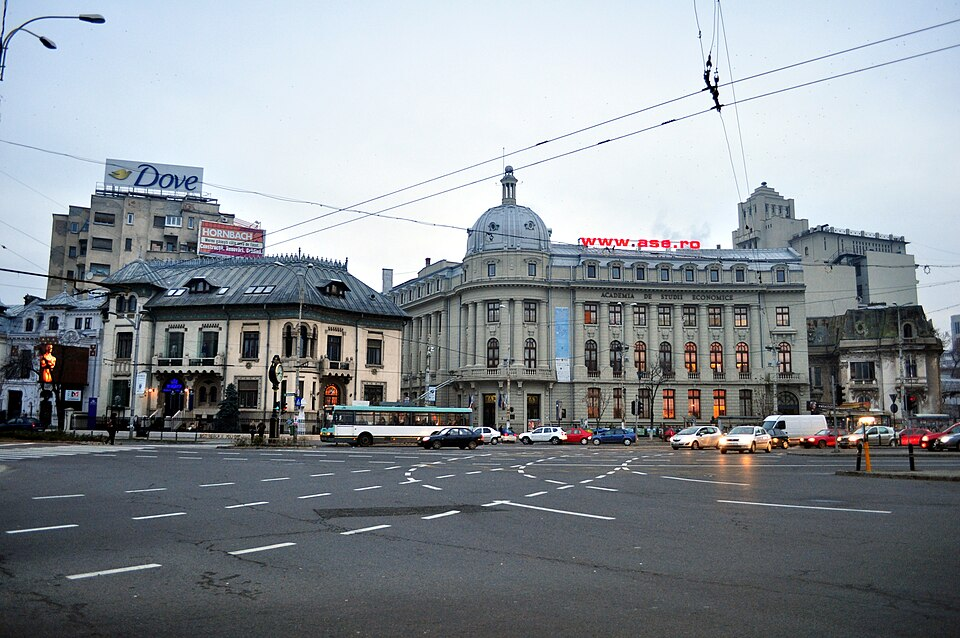
\includegraphics[height=0.40\textheight]{ch0_ase_2014.jpg}\\[1mm]
\imgcap{Academia de Studii Economice din București}
\imgcredit{https://commons.wikimedia.org/wiki/File:Bucharest_-_Academie_de_Studii_Economice_01.jpg}{Foto: Joe Mabel (2014); CC BY 3.0; Wikimedia Commons}
\end{column}
\end{columns}
\end{frame}

\begin{frame}{Rezultatele învățării}
\itemsize{\small}
\begin{itemize}
    \item Situați fiecare capitol pe drumul de la descrierea unei serii la modelarea și prognoza ei
    \item Reamintiți formula-cheie, faptul empiric principal și greșeala cea mai frecventă din fiecare capitol
    \item Alegeți testul sau modelul potrivit pentru o întrebare dată despre o serie de timp
    \item Aplicați metoda Box--Jenkins pe o serie reală: transformare, testare, identificare, estimare, verificare, prognoză
    \item Citiți rezultatele obținute cu software (estimări, teste, corelograme) și interpretați-le în trei pînă la cinci fraze
    \item Planificați proiectul de echipă, susținerea orală și declararea utilizării AI
\end{itemize}
\end{frame}

\begin{frame}{Bibliografie și instrumente}
\itemsize{\small}
\begin{itemize}
    \item Manual: \refHP; manual însoțitor gratuit: \refFPP
    \begin{itemize}
        \item teorie: \refBD; \refHamilton; metoda: \refBJ
    \end{itemize}
    \item Quantlet-urile Python ale capitolului: \href{https://github.com/danpele/Time-Series-Analysis/tree/main/Quantlets/Ch_15}{Quantlets/Ch\_15}
    \begin{itemize}
        \item cazul Box--Jenkins pe IAPC-ul României și rezultatele pentru problema 3 de examen
    \end{itemize}
    \item Notebook-ul cursului, cursul într-un singur notebook: \href{\colaburl{notebooks/EN/chapter15_lecture_notebook.ipynb}}{deschideți în Google Colab}
    \item Autoevaluare: quiz-ul acestui capitol, 20 de întrebări extrase din toate capitolele
\end{itemize}
\end{frame}


%=============================================================================
\section{Harta cursului}
%=============================================================================

\begin{frame}{Harta cursului: \tsachlinkt{https://danpele.github.io/Time-Series-Analysis/RO/Cursuri/capitol0_introducere.pdf}{Capitolele 0}--\tsachlinkt{https://danpele.github.io/Time-Series-Analysis/RO/Cursuri/capitol14_modele_garch_multivariate.pdf}{14}}
\itemsize{\footnotesize}
\begin{center}
\resizebox{0.97\textwidth}{!}{%
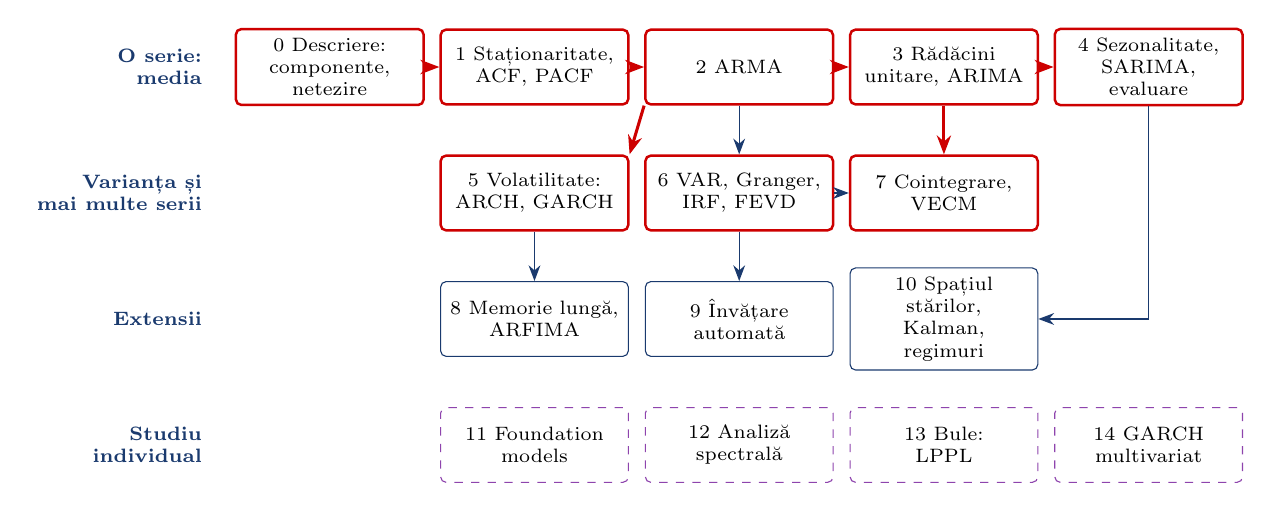
\begin{tikzpicture}[
  box/.style={draw=MainBlue, rounded corners=2pt, fill=white, font=\scriptsize, align=center, minimum height=0.95cm, text width=2.15cm},
  key/.style={box, draw=IDAred, line width=0.9pt},
  self/.style={box, dashed, draw=Purple},
  lab/.style={font=\scriptsize\bfseries, text=MainBlue, anchor=east, align=right},
  arr/.style={-{Stealth[length=2mm]}, MainBlue, line width=0.5pt},
  karr/.style={-{Stealth[length=2.4mm]}, IDAred, line width=1.1pt},
  sarr/.style={-{Stealth[length=2mm]}, Purple, dashed, line width=0.5pt}]
\node[lab] at (-0.2, 0) {O serie:\\ media};
\node[key] (c0) at (1.3, 0) {0 Descriere:\\ componente, netezire};
\node[key] (c1) at (3.9, 0) {1 Staționaritate,\\ ACF, PACF};
\node[key] (c2) at (6.5, 0) {2 ARMA};
\node[key] (c3) at (9.1, 0) {3 Rădăcini\\ unitare, ARIMA};
\node[key] (c4) at (11.7, 0) {4 Sezonalitate,\\ SARIMA, evaluare};
\node[lab] at (-0.2, -1.6) {Varianța și\\ mai multe serii};
\node[key] (c5) at (3.9, -1.6) {5 Volatilitate:\\ ARCH, GARCH};
\node[key] (c6) at (6.5, -1.6) {6 VAR, Granger,\\ IRF, FEVD};
\node[key] (c7) at (9.1, -1.6) {7 Cointegrare,\\ VECM};
\node[lab] at (-0.2, -3.2) {Extensii};
\node[box] (c8) at (3.9, -3.2) {8 Memorie lungă,\\ ARFIMA};
\node[box] (c9) at (6.5, -3.2) {9 Învățare\\ automată};
\node[box] (c10) at (9.1, -3.2) {10 Spațiul stărilor,\\ Kalman, regimuri};
\node[lab] at (-0.2, -4.8) {Studiu\\ individual};
\node[self] (c11) at (3.9, -4.8) {11 Foundation\\ models};
\node[self] (c12) at (6.5, -4.8) {12 Analiză\\ spectrală};
\node[self] (c13) at (9.1, -4.8) {13 Bule:\\ LPPL};
\node[self] (c14) at (11.7, -4.8) {14 GARCH\\ multivariat};
\draw[karr] (c0) -- (c1); \draw[karr] (c1) -- (c2); \draw[karr] (c2) -- (c3); \draw[karr] (c3) -- (c4);
\draw[karr] (c2.south west) -- (c5.north east); \draw[karr] (c3) -- (c7); \draw[arr] (c2) -- (c6); \draw[arr] (c6) -- (c7);
\draw[arr] (c5) -- (c8); \draw[arr] (c6) -- (c9); \draw[arr] (c4.south) -- (11.7, -3.2) -- (c10.east);
\end{tikzpicture}}
\end{center}
\vspace{-0.2cm}
\begin{itemize}
    \item Roșu: nucleul examenului, de la descrierea unei serii la modelarea împreună a mai multor serii
    \item Albastru: extensii (\tsachlink{https://danpele.github.io/Time-Series-Analysis/RO/Cursuri/capitol8_memorie_lunga_arfima.pdf}{Capitolele 8}--\tsachlink{https://danpele.github.io/Time-Series-Analysis/RO/Cursuri/capitol10_spatiul_starilor_kalman_markov_switching.pdf}{10}); linie întreruptă: studiu individual (\tsachlink{https://danpele.github.io/Time-Series-Analysis/RO/Cursuri/capitol11_foundation_models_serii_timp.pdf}{Capitolele 11}--\tsachlink{https://danpele.github.io/Time-Series-Analysis/RO/Cursuri/capitol14_modele_garch_multivariate.pdf}{14}), fiecare construit pe un capitol de bază: 11 pe 9, 12 pe 1 și 8, 13 pe 3, 14 pe 5 și 6
\end{itemize}
\end{frame}

\begin{frame}{Seriile cursului}
\itemsize{\small}
\begin{center}
\footnotesize
\begin{tabular}{>{\raggedright\arraybackslash}p{3.6cm}>{\raggedright\arraybackslash}p{2.6cm}>{\raggedright\arraybackslash}p{4.2cm}l}
\toprule
\textbf{Seria} & \textbf{Sursa} & \textbf{Tema ilustrată} & \textbf{Cap.} \\
\midrule
PIB-ul real al României (trimestrial) & Eurostat & trend, sezonalitate, rădăcină unitară, regimuri & 0--4, 10 \\
Inflația IAPC a României (lunar) & Eurostat & persistență, sezonalitate, memorie lungă & 2--4, 8 \\
ROBOR 3M, șomaj & Eurostat & un VAR pentru economia României & 6 \\
EUR/RON & BNR & un mers aleator greu de depășit & 0, 3, 5 \\
BET, S\&P 500, DAX (zilnic) & EODHD & volatility clustering, spillover & 1, 5, 6 \\
consumul de electricitate (zilnic, orar) & ENTSO-E & sezonalitate multiplă, învățare automată & 4, 9 \\
Nilul, petele solare, randamentele și PIB-ul SUA & statsmodels, FRED & exemplele clasice ale manualelor & 1, 2, 7, 8, 10 \\
\bottomrule
\end{tabular}
\end{center}
\begin{itemize}
    \item Fiecare cifră de pe slide-urile de recapitulare este cifra din capitolul ei: aceleași date, aceeași fereastră, același cod
\end{itemize}
\end{frame}


%=============================================================================
\section{Capitolele 0--3: descriere, staționaritate, ARMA, ARIMA}
%=============================================================================

\begin{frame}{\tsachlinkt{https://danpele.github.io/Time-Series-Analysis/RO/Cursuri/capitol0_introducere.pdf}{Capitolul 0}: introducere: componente și netezire exponențială}
\itemsize{\footnotesize}
\begin{itemize}
    \item \textbf{Formule-cheie}
    \begin{itemize}
        \item aditiv $y_t = T_t + S_t + R_t$ sau multiplicativ $y_t = T_t S_t R_t$; logaritmul transformă un model în celălalt
        \item SES $\ell_t = \alpha y_t + (1 - \alpha)\ell_{t-1}$; MASE $=$ MAE $/$ MAE metodei naive sezoniere în eșantion
    \end{itemize}
    \item \textbf{Fapte empirice}
    \begin{itemize}
        \item PIB-ul României a crescut de 2{,}3 ori din 1995 (2{,}8\% pe an); trimestrul I este cu circa $\ensuremath{-}23{,}8\%$, iar trimestrul IV cu $+20{,}7\%$ față de trend
        \item EUR/RON: $\hat\alpha_{SES} = 1{,}00$, ultima valoare este cea mai bună prognoză; electricitatea: Holt--Winters are MASE 0{,}51, față de 0{,}82 pentru metoda naivă
    \end{itemize}
    \item \textbf{Greșeli frecvente}
    \begin{itemize}
        \item judecarea unei prognoze pe datele folosite la estimare
        \item MAPE pentru serii care trec prin zero (inflația lunară); un model aditiv pentru o oscilație sezonieră care crește odată cu nivelul
    \end{itemize}
\end{itemize}
\end{frame}

\begin{frame}{\tsachlinkt{https://danpele.github.io/Time-Series-Analysis/RO/Cursuri/capitol1_procese_stochastice_stationaritate.pdf}{Capitolul 1}: procese stochastice și staționaritate}
\itemsize{\footnotesize}
\begin{itemize}
    \item \textbf{Formule-cheie}
    \begin{itemize}
        \item staționaritate slabă: $E X_t = \mu$, $\mathrm{Cov}(X_t, X_{t+h}) = \gamma(h)$; $\hat\rho(h)$ comparat cu $\pm 1{,}96/\sqrt{T}$
        \item Ljung--Box $Q^*(m) = T(T + 2)\sum_{h=1}^{m}\hat\rho(h)^2/(T - h) \sim \chi^2(m)$ \refLB; mers aleator $\mathrm{Var}(X_t) = t\sigma^2$
    \end{itemize}
    \item \textbf{Fapte empirice}
    \begin{itemize}
        \item randamentele BET: $\hat\rho_1 = 0{,}11$, randamentele absolute $\hat\rho_1 = 0{,}40$ (banda $\pm 0{,}024$): necorelat nu înseamnă independent
        \item PIB-ul României: Box--Cox $\hat\lambda = 0{,}02$, adică logaritmul; o diferențiere în plus dă $\hat\rho_1 = \ensuremath{-}0{,}54$
    \end{itemize}
    \item \textbf{Greșeli frecvente}
    \begin{itemize}
        \item interpretarea unei singure bare din afara benzii ca semnal (una din douăzeci iese din întîmplare)
        \item diferențierea unei serii care este deja staționară
    \end{itemize}
\end{itemize}
\end{frame}

\begin{frame}{\tsachlinkt{https://danpele.github.io/Time-Series-Analysis/RO/Cursuri/capitol2_modele_arma.pdf}{Capitolul 2}: modele ARMA}
\itemsize{\footnotesize}
\begin{itemize}
    \item \textbf{Formule-cheie}
    \begin{itemize}
        \item $\phi(L)(X_t - \mu) = \theta(L)\varepsilon_t$; AR(1) $\rho(h) = \phi^h$; MA(1) $\rho(1) = \theta/(1 + \theta^2)$
        \item AIC $= -2\ln L + 2k$ \refAkaike, BIC $= -2\ln L + k\ln T$ \refSchwarz; verificarea reziduurilor $Q^*(m) \sim \chi^2(m - p - q)$
    \end{itemize}
    \item \textbf{Fapte empirice}
    \begin{itemize}
        \item creșterea anuală a PIB-ului României: MA(3) după BIC, efectul trimestrelor suprapuse; Ljung--Box pe reziduuri $p = 0{,}37$
        \item inflația din România: AR(2) cu $\hat\phi_1 + \hat\phi_2 = 0{,}976$, aproape de o rădăcină unitară; petele solare: un ciclu AR(2) de 10{,}6 ani
    \end{itemize}
    \item \textbf{Greșeli frecvente}
    \begin{itemize}
        \item citirea ordinului AR din ACF (la un AR se anulează PACF)
        \item Ljung--Box pe reziduuri cu $m$ în loc de $m - p - q$ grade de libertate; un factor comun în $\phi(L)$ și $\theta(L)$
    \end{itemize}
\end{itemize}
\end{frame}

\begin{frame}{\tsachlinkt{https://danpele.github.io/Time-Series-Analysis/RO/Cursuri/capitol3_radacini_unitare_modele_arima.pdf}{Capitolul 3}: rădăcini unitare și modele ARIMA}
\itemsize{\footnotesize}
\begin{itemize}
    \item \textbf{Formule-cheie}
    \begin{itemize}
        \item ADF: $\Delta y_t = c + bt + \gamma y_{t-1} + \sum_j\delta_j\Delta y_{t-j} + \varepsilon_t$, $H_0$: $\gamma = 0$ \refDF; KPSS: $H_0$ staționaritate \refKPSS
        \item ARIMA$(p,d,q)$: $\phi(L)(1 - L)^d y_t = c + \theta(L)\varepsilon_t$; varianța prognozei crește cu $h$ cînd $d \ge 1$
    \end{itemize}
    \item \textbf{Fapte empirice}
    \begin{itemize}
        \item logaritmul PIB-ului României: $\tau = \ensuremath{-}2{,}31$ ($p = 0{,}43$, valoarea critică la 5\% $\ensuremath{-}3{,}45$); creșterea: $\tau = \ensuremath{-}10{,}77$; ARIMA(0,1,0) cu derivă de 0{,}81\% pe trimestru
        \item două mersuri aleatoare independente: un $t$ semnificativ în 90\% din regresii \refGN; puterea ADF doar 12{,}5\% pentru $\phi = 0{,}95$, $T = 100$
    \end{itemize}
    \item \textbf{Greșeli frecvente}
    \begin{itemize}
        \item valori critice Student sau Normale pentru statistica ADF
        \item interpretarea nerespingerii ca dovadă a rădăcinii unitare; o regresie în niveluri între serii $I(1)$ fără test de cointegrare
    \end{itemize}
\end{itemize}
\end{frame}

\begin{frame}{Recapitulare: \tsachlinkt{https://danpele.github.io/Time-Series-Analysis/RO/Cursuri/capitol0_introducere.pdf}{capitolele 0}--\tsachlinkt{https://danpele.github.io/Time-Series-Analysis/RO/Cursuri/capitol3_radacini_unitare_modele_arima.pdf}{3}}
\itemsize{\small}
\begin{itemize}
    \item Întîi graficul, apoi transformarea: logaritm pentru o oscilație care crește, diferențe pentru un trend stochastic
    \item ACF și PACF identifică un ARMA; AIC și BIC aleg; Ljung--Box pe reziduuri verifică
    \item ADF și KPSS împreună decid $d$; valori critice Dickey--Fuller, niciodată Student
\end{itemize}
\end{frame}


%=============================================================================
\section{Capitolele 4--7: sezonalitate, volatilitate, VAR, VECM}
%=============================================================================

\begin{frame}{\tsachlinkt{https://danpele.github.io/Time-Series-Analysis/RO/Cursuri/capitol4_sezonalitate_prognoza.pdf}{Capitolul 4}: sezonalitate și prognoză}
\itemsize{\footnotesize}
\begin{itemize}
    \item \textbf{Formule-cheie}
    \begin{itemize}
        \item SARIMA $\phi(L)\Phi(L^s)(1 - L)^d(1 - L^s)^D y_t = \theta(L)\Theta(L^s)\varepsilon_t$; airline $(0,1,1)(0,1,1)_s$
        \item Diebold--Mariano $\bar d/\sqrt{\hat V/n}$, $d_t = L(e_{1t}) - L(e_{2t})$ \refDM, cu corecția HLN \refHLN
    \end{itemize}
    \item \textbf{Fapte empirice}
    \begin{itemize}
        \item pasagerii aerieni: MAPE 8{,}5\% pentru modelul airline, față de 15{,}5\% pentru metoda naivă sezonieră
        \item Paștele ortodox crește vînzările de alimente din România cu circa 5{,}9\%; consumul zilnic: DHR are MASE 0{,}89, față de 1{,}28 (naiv sezonier)
    \end{itemize}
    \item \textbf{Greșeli frecvente}
    \begin{itemize}
        \item compararea AICc pentru modele cu $d$ sau $D$ diferite
        \item judecarea prognozelor la o singură origine; date ajustate sezonier într-o prognoză SARIMA a datelor brute
    \end{itemize}
\end{itemize}
\end{frame}

\begin{frame}{\tsachlinkt{https://danpele.github.io/Time-Series-Analysis/RO/Cursuri/capitol5_volatilitate_conditionata_garch.pdf}{Capitolul 5}: volatilitate condiționată: ARCH și GARCH}
\itemsize{\footnotesize}
\begin{itemize}
    \item \textbf{Formule-cheie}
    \begin{itemize}
        \item GARCH(1,1) $\sigma_t^2 = \omega + \alpha\varepsilon_{t-1}^2 + \beta\sigma_{t-1}^2$ \refEngle, \refBoll; $\bar\sigma^2 = \omega/(1 - \alpha - \beta)$, $h_{1/2} = \ln 0{,}5/\ln(\alpha + \beta)$
        \item ARCH-LM $= nR^2 \sim \chi^2(q)$; VaR 1\% $= -(\mu + \sigma_{t+1}q_{0{,}01}(z))$
    \end{itemize}
    \item \textbf{Fapte empirice}
    \begin{itemize}
        \item GARCH(1,1)-$t$: $\alpha + \beta = 0{,}995$ pentru S\&P 500 (timp de înjumătățire 131 de zile), $0{,}991$ pentru BET (74 de zile)
        \item S\&P 500: GJR $\hat\gamma = 0{,}21$ ($t = 10{,}0$); coeficientul de boltire 13{,}7 pentru randamente, 5{,}0 pentru reziduurile standardizate
    \end{itemize}
    \item \textbf{Greșeli frecvente}
    \begin{itemize}
        \item timpul de înjumătățire scris $1/(1 - \alpha - \beta)$; o varianță pe termen lung raportată cînd $\alpha + \beta \ge 1$
        \item „VaR 99\%” sau un VaR negativ: în curs scriem VaR 1\%, o pierdere pozitivă
    \end{itemize}
\end{itemize}
\end{frame}

\begin{frame}{\tsachlinkt{https://danpele.github.io/Time-Series-Analysis/RO/Cursuri/capitol6_modele_var_cauzalitate_granger.pdf}{Capitolul 6}: modele VAR și cauzalitate Granger}
\itemsize{\footnotesize}
\begin{itemize}
    \item \textbf{Formule-cheie}
    \begin{itemize}
        \item VAR$(p)$: $\bY_t = \bc + \bA_1\bY_{t-1} + \dots + \bA_p\bY_{t-p} + \bepsilon_t$ \refSims; stabil dacă toate valorile proprii ale matricei companion sînt în interiorul cercului unitate
        \item Granger $F = [(RSS_R - RSS_U)/p]\,/\,[RSS_U/(T - Kp - 1)]$ \refGranger; IRF și FEVD cu o ordine Cholesky
    \end{itemize}
    \item \textbf{Fapte empirice}
    \begin{itemize}
        \item VAR(2) pentru România (creștere, inflație, ROBOR 3M): creșterea cauzează Granger ROBOR, $F = 7{,}26$, $p =$ 0{,}001
        \item spillover între S\&P 500, DAX și BET: în medie 26{,}4\%, 57{,}5\% la 17 martie 2020
    \end{itemize}
    \item \textbf{Greșeli frecvente}
    \begin{itemize}
        \item interpretarea cauzalității Granger drept cauzalitate (este doar predictibilitate suplimentară)
        \item IRF raportate fără ordinea care stă la baza lor; prea multe decalaje pentru un eșantion scurt
    \end{itemize}
\end{itemize}
\end{frame}

\begin{frame}{\tsachlinkt{https://danpele.github.io/Time-Series-Analysis/RO/Cursuri/capitol7_cointegrare_vecm.pdf}{Capitolul 7}: cointegrare și VECM}
\itemsize{\footnotesize}
\begin{itemize}
    \item \textbf{Formule-cheie}
    \begin{itemize}
        \item Engle--Granger: OLS în niveluri, apoi ADF pe reziduuri cu valorile critice MacKinnon \refEG; timpul de înjumătățire al ECM $\ln 0{,}5/\ln(1 + \gamma)$
        \item VECM $\Delta\mathbf y_t = \alpha\beta^\top\mathbf y_{t-1} + \sum_i\Gamma_i\Delta\mathbf y_{t-i} + \mathbf u_t$; statistica urmei $-T\sum_{i>r}\ln(1 - \hat\lambda_i)$ \refJoh
    \end{itemize}
    \item \textbf{Fapte empirice}
    \begin{itemize}
        \item randamentele SUA la 1, 5 și 10 ani: urma 54{,}6 $>$ 29{,}8 pentru $r = 0$, 3{,}12 $<$ 3{,}84 pentru $r \le 2$: rangul 2; timpul de înjumătățire al ECM pentru dobînda lungă 20{,}8 luni
        \item PPP pentru leu: ADF $p = 0{,}24$ pentru cursul real, nestaționar; pairs trading la BVB: Sharpe 0{,}15 brut, 0{,}05 net
    \end{itemize}
    \item \textbf{Greșeli frecvente}
    \begin{itemize}
        \item valorile critice Dickey--Fuller pentru reziduurile Engle--Granger (trebuie să fie mai negative)
        \item un VAR în diferențe pentru serii cointegrate (omite termenul de corecție a erorii)
    \end{itemize}
\end{itemize}
\end{frame}

\begin{frame}{Recapitulare: \tsachlinkt{https://danpele.github.io/Time-Series-Analysis/RO/Cursuri/capitol4_sezonalitate_prognoza.pdf}{capitolele 4}--\tsachlinkt{https://danpele.github.io/Time-Series-Analysis/RO/Cursuri/capitol7_cointegrare_vecm.pdf}{7}}
\itemsize{\small}
\begin{itemize}
    \item Sezonalitatea: $\Delta_s$ sau termeni Fourier; efectele de calendar ca regresori; evaluare cu origini mobile, MASE și DM
    \item Volatilitatea: ARCH-LM, apoi GARCH(1,1)-$t$; persistență aproape de 1; VaR 1\% cu cuantila potrivită
    \item Mai multe serii: VAR pentru date staționare, VECM pentru date $I(1)$ cointegrate; Granger înseamnă predictibilitate
\end{itemize}
\end{frame}


%=============================================================================
\section{Capitolele 8--10: memorie lungă, învățare automată, spațiul stărilor}
%=============================================================================

\begin{frame}{\tsachlinkt{https://danpele.github.io/Time-Series-Analysis/RO/Cursuri/capitol8_memorie_lunga_arfima.pdf}{Capitolul 8}: memorie lungă și ARFIMA}
\itemsize{\footnotesize}
\begin{itemize}
    \item \textbf{Formule-cheie}
    \begin{itemize}
        \item $(1 - L)^d$ cu $\pi_k = \pi_{k-1}(k - 1 - d)/k$ \refGJ, \refHosking; $\rho(k) \sim Ck^{2d-1}$; $H = d + 1/2$
        \item staționar pentru $d < 1/2$, cu revenire la medie pentru $d < 1$; GPH și Whittle local folosesc cele mai joase $m$ frecvențe
    \end{itemize}
    \item \textbf{Fapte empirice}
    \begin{itemize}
        \item inflația lunară din România: ARFIMA(0,$d$,0) cu $\hat d = 0{,}31$ (SE 0{,}05) bate ARMA după AIC și BIC
        \item S\&P 500: $H$ (R/S) 0{,}53 pentru randamente, 0{,}86 pentru $|r_t|$; Nilul: $\hat d = 0{,}40$, dar $\ensuremath{-}0{,}17$ după ruptura din 1898
    \end{itemize}
    \item \textbf{Greșeli frecvente}
    \begin{itemize}
        \item o ruptură sau o schimbare de regim interpretată drept memorie lungă
        \item o singură lățime de bandă $m$; memoria lungă a randamentelor confundată cu memoria lungă a volatilității
    \end{itemize}
\end{itemize}
\end{frame}

\begin{frame}{\tsachlinkt{https://danpele.github.io/Time-Series-Analysis/RO/Cursuri/capitol9_invatare_automata_serii_timp.pdf}{Capitolul 9}: învățare automată pentru serii de timp}
\itemsize{\footnotesize}
\begin{itemize}
    \item \textbf{Formule-cheie}
    \begin{itemize}
        \item prognoza directă $\hat y_{T+h} = \hat f_h(y_T, \dots, y_{T-p+1}, \mathbf z_{T+h})$; ridge $+\lambda\sum\beta_j^2$, lasso $+\lambda\sum|\beta_j|$
        \item deplasare--varianță $E(y_0 - \hat f)^2 = \text{deplasare}^2 + \mathrm{Var}(\hat f) + \sigma^2$; doar validare walk-forward
    \end{itemize}
    \item \textbf{Fapte empirice}
    \begin{itemize}
        \item S\&P 500, același model: $R^2 = 0{,}37$ cu $k$-fold aleator, $\ensuremath{-}0{,}39$ walk-forward: scurgere de informație
        \item semnul randamentelor: clasa majoritară 54{,}4\%, boosting 52{,}5\%; consumul zilnic: ridge MASE 0{,}90, LSTM 1{,}16 \refMfour
    \end{itemize}
    \item \textbf{Greșeli frecvente}
    \begin{itemize}
        \item validarea încrucișată aleatoare și scalarea pe tot eșantionul (look-ahead)
        \item arbori pe niveluri cu trend (nu pot extrapola); comparații fără un reper simplu
    \end{itemize}
\end{itemize}
\end{frame}

\begin{frame}{\tsachlinkt{https://danpele.github.io/Time-Series-Analysis/RO/Cursuri/capitol10_spatiul_starilor_kalman_markov_switching.pdf}{Capitolul 10}: spațiul stărilor, filtrul Kalman și modele Markov switching}
\itemsize{\footnotesize}
\begin{itemize}
    \item \textbf{Formule-cheie}
    \begin{itemize}
        \item $y_t = Z\alpha_t + \varepsilon_t$, $\alpha_{t+1} = T\alpha_t + R\eta_t$; $K_t = P_tZ'F_t^{-1}$, $a_{t|t} = a_t + K_tv_t$ \refKalman
        \item Markov switching: durate $1/(1 - p_{ii})$, ergodic $\pi_1 = (1 - p_{22})/(2 - p_{11} - p_{22})$ \refHamMS
    \end{itemize}
    \item \textbf{Fapte empirice}
    \begin{itemize}
        \item Nilul: $\hat q = 0{,}097$, cîștigul de echilibru $\bar K = 0{,}267$, ponderea netezirii exponențiale
        \item PIB-ul SUA: regimurile coincid cu datările NBER în 90\% din trimestre; PIB-ul României: regimul stabil 15{,}2 trimestre, cel volatil 11{,}2
    \end{itemize}
    \item \textbf{Greșeli frecvente}
    \begin{itemize}
        \item probabilități netezite folosite ca și cum ar fi fost cunoscute în timp real
        \item durate scrise $p_{ii}/(1 - p_{ii})$; ultima valoare a deviației HP interpretată ca estimare în timp real
    \end{itemize}
\end{itemize}
\end{frame}

\begin{frame}{Recapitulare: \tsachlinkt{https://danpele.github.io/Time-Series-Analysis/RO/Cursuri/capitol8_memorie_lunga_arfima.pdf}{capitolele 8}--\tsachlinkt{https://danpele.github.io/Time-Series-Analysis/RO/Cursuri/capitol10_spatiul_starilor_kalman_markov_switching.pdf}{10}}
\itemsize{\small}
\begin{itemize}
    \item Memoria lungă: ACF hiperbolică, $d$ între 0 și 1/2; verificați rupturile și regimurile înainte de a o accepta
    \item Învățarea automată: același tabel supervizat, validare walk-forward, repere simple
    \item Spațiul stărilor: filtrul Kalman pentru niveluri și trenduri ascunse; Markov switching pentru regimuri
\end{itemize}
\end{frame}


%=============================================================================
\section{Capitolele 11--14: studiu individual}
%=============================================================================

\begin{frame}{\tsachlinkt{https://danpele.github.io/Time-Series-Analysis/RO/Cursuri/capitol11_foundation_models_serii_timp.pdf}{Capitolul 11}: foundation models pentru serii de timp (studiu individual)}
\itemsize{\footnotesize}
\begin{itemize}
    \item \textbf{Idei principale}
    \begin{itemize}
        \item modele transformer pre-antrenate pe foarte multe serii: tokenizarea și împărțirea valorilor în segmente (patching)
        \item Chronos, TimesFM, Moirai, Lag-Llama: prognoze zero-shot și fine-tuning
        \item o comparație corectă: același eșantion de test, MASE, scoruri probabilistice, repere simple
    \end{itemize}
    \item \textbf{Legătura cu nucleul cursului}
    \begin{itemize}
        \item un model global pe multe serii (\tsachlink{https://danpele.github.io/Time-Series-Analysis/RO/Cursuri/capitol9_invatare_automata_serii_timp.pdf}{Capitolul 9}); evaluat ca orice prognoză (\tsachlink{https://danpele.github.io/Time-Series-Analysis/RO/Cursuri/capitol4_sezonalitate_prognoza.pdf}{Capitolul 4})
    \end{itemize}
    \item \tsachlink{https://danpele.github.io/Time-Series-Analysis/RO/Cursuri/capitol11_foundation_models_serii_timp.pdf}{Capitolele 11}--\tsachlink{https://danpele.github.io/Time-Series-Analysis/RO/Cursuri/capitol14_modele_garch_multivariate.pdf}{14} sînt pentru studiu individual (nu se examinează, dacă titularul nu decide altfel)
\end{itemize}
\end{frame}

\begin{frame}{\tsachlinkt{https://danpele.github.io/Time-Series-Analysis/RO/Cursuri/capitol12_analiza_spectrala.pdf}{Capitolul 12}: analiză spectrală (studiu individual)}
\itemsize{\footnotesize}
\begin{itemize}
    \item \textbf{Idei principale}
    \begin{itemize}
        \item transformata Fourier, periodograma $I(\lambda_j)$ și densitatea spectrală
        \item periodograme netezite (Welch), filtre (Hodrick--Prescott) și ciclul economic
        \item coerența dintre două serii; wavelets ca instrument timp--frecvență
    \end{itemize}
    \item \textbf{Legătura cu nucleul cursului}
    \begin{itemize}
        \item aceeași informație ca ACF, pe frecvențe (\tsachlink{https://danpele.github.io/Time-Series-Analysis/RO/Cursuri/capitol1_procese_stochastice_stationaritate.pdf}{Capitolul 1}); polul spectral al memoriei lungi (\tsachlink{https://danpele.github.io/Time-Series-Analysis/RO/Cursuri/capitol8_memorie_lunga_arfima.pdf}{Capitolul 8})
    \end{itemize}
    \item \tsachlink{https://danpele.github.io/Time-Series-Analysis/RO/Cursuri/capitol11_foundation_models_serii_timp.pdf}{Capitolele 11}--\tsachlink{https://danpele.github.io/Time-Series-Analysis/RO/Cursuri/capitol14_modele_garch_multivariate.pdf}{14} sînt pentru studiu individual (nu se examinează, dacă titularul nu decide altfel)
\end{itemize}
\end{frame}

\begin{frame}{\tsachlinkt{https://danpele.github.io/Time-Series-Analysis/RO/Cursuri/capitol13_bule_lppl.pdf}{Capitolul 13}: bule speculative: modele LPPL (studiu individual)}
\itemsize{\footnotesize}
\begin{itemize}
    \item \textbf{Idei principale}
    \begin{itemize}
        \item bulele ca o creștere superexponențială a prețurilor
        \item modelul LPPLS: o lege putere plus oscilații log-periodice; estimare și condiții de filtrare
        \item indicatorul de încredere LPPLS pe bule și crahuri istorice
    \end{itemize}
    \item \textbf{Legătura cu nucleul cursului}
    \begin{itemize}
        \item rădăcini explozive, opusul rădăcinilor unitare (\tsachlink{https://danpele.github.io/Time-Series-Analysis/RO/Cursuri/capitol3_radacini_unitare_modele_arima.pdf}{Capitolul 3}); volatilitatea dinaintea crahurilor (\tsachlink{https://danpele.github.io/Time-Series-Analysis/RO/Cursuri/capitol5_volatilitate_conditionata_garch.pdf}{Capitolul 5})
    \end{itemize}
    \item \tsachlink{https://danpele.github.io/Time-Series-Analysis/RO/Cursuri/capitol11_foundation_models_serii_timp.pdf}{Capitolele 11}--\tsachlink{https://danpele.github.io/Time-Series-Analysis/RO/Cursuri/capitol14_modele_garch_multivariate.pdf}{14} sînt pentru studiu individual (nu se examinează, dacă titularul nu decide altfel)
\end{itemize}
\end{frame}

\begin{frame}{\tsachlinkt{https://danpele.github.io/Time-Series-Analysis/RO/Cursuri/capitol14_modele_garch_multivariate.pdf}{Capitolul 14}: modele GARCH multivariate (studiu individual)}
\itemsize{\footnotesize}
\begin{itemize}
    \item \textbf{Idei principale}
    \begin{itemize}
        \item covarianțe și corelații variabile în timp; numărul de parametri crește foarte repede
        \item VEC, BEKK, CCC și DCC; estimarea DCC în doi pași
        \item corelații dinamice, varianța portofoliului și VaR 1\%
    \end{itemize}
    \item \textbf{Legătura cu nucleul cursului}
    \begin{itemize}
        \item GARCH pentru fiecare serie (\tsachlink{https://danpele.github.io/Time-Series-Analysis/RO/Cursuri/capitol5_volatilitate_conditionata_garch.pdf}{Capitolul 5}) și perspectiva multivariată a VAR (\tsachlink{https://danpele.github.io/Time-Series-Analysis/RO/Cursuri/capitol6_modele_var_cauzalitate_granger.pdf}{Capitolul 6})
    \end{itemize}
    \item \tsachlink{https://danpele.github.io/Time-Series-Analysis/RO/Cursuri/capitol11_foundation_models_serii_timp.pdf}{Capitolele 11}--\tsachlink{https://danpele.github.io/Time-Series-Analysis/RO/Cursuri/capitol14_modele_garch_multivariate.pdf}{14} sînt pentru studiu individual (nu se examinează, dacă titularul nu decide altfel)
\end{itemize}
\end{frame}


%=============================================================================
\section{Trusa de instrumente}
%=============================================================================

\begin{frame}{Trusa de instrumente (1/2): o serie, media}
\itemsize{\small}
\begin{center}
\footnotesize
\begin{tabular}{>{\raggedright\arraybackslash}p{3.5cm}>{\raggedright\arraybackslash}p{3.5cm}>{\raggedright\arraybackslash}p{3.6cm}c}
\toprule
\textbf{Întrebarea} & \textbf{Instrumentul} & \textbf{Decizia} & \textbf{Cap.} \\
\midrule
Este seria staționară? & grafic, ACF; ADF și KPSS & ADF respinge, KPSS nu: staționară & 1, 3 \\
Trend: determinist sau stochastic? & ADF și KPSS cu trend & eliminarea trendului sau diferențierea & 3 \\
Există sezonalitate? & graficul sezonier, ACF la $s$, $2s$; OCSB, HEGY & $\Delta_s$ sau variabile dummy și termeni Fourier & 4 \\
Ce model ARMA? & ACF, PACF; AIC, BIC & cel mai mic BIC cu reziduuri zgomot alb & 2 \\
Sînt reziduurile adecvate? & Ljung--Box cu $m - k$ grade de libertate; Jarque--Bera & $p > 0{,}05$: nu mai rămîne autocorelație & 2 \\
Care prognoză este mai bună? & eșantion de test, origini mobile; MASE, DM & DM cu $p < 0{,}05$; altfel egalitate & 0, 4 \\
\bottomrule
\end{tabular}
\end{center}
\end{frame}

\begin{frame}{Trusa de instrumente (2/2): varianță, mai multe serii, extensii}
\itemsize{\small}
\begin{center}
\footnotesize
\begin{tabular}{>{\raggedright\arraybackslash}p{3.5cm}>{\raggedright\arraybackslash}p{3.5cm}>{\raggedright\arraybackslash}p{3.6cm}c}
\toprule
\textbf{Întrebarea} & \textbf{Instrumentul} & \textbf{Decizia} & \textbf{Cap.} \\
\midrule
Se schimbă varianța? & Ljung--Box pe $r_t^2$, ARCH-LM & respingem: GARCH(1,1)-$t$, GJR & 5 \\
Ajută $x$ la prognoza lui $y$? & VAR, testul Granger $F$ & $p < 0{,}05$: cauzalitate Granger & 6 \\
Ce efect are un șoc? & IRF, FEVD (Cholesky) & benzi bootstrap; încercați alte ordini & 6 \\
Există un echilibru pe termen lung? & Engle--Granger, Johansen & VECM: $\beta$, $\alpha$, timpul de înjumătățire & 7 \\
Memorie lungă? & GPH, Whittle local, ARFIMA & mai multe valori $m$; verificați rupturile & 8 \\
Mulți predictori, efecte neliniare? & ridge, lasso, arbori, boosting & walk-forward față de un reper & 9 \\
Un nivel sau un regim ascuns? & filtrul Kalman, Markov switching & filtrat pentru timp real, netezit pentru istorie & 10 \\
\bottomrule
\end{tabular}
\end{center}
\end{frame}

\begin{frame}{Convențiile folosite în tot cursul}
\itemsize{\small}
\begin{itemize}
    \item \textbf{Transformările}: $100\ln y_t$; creșterea $100\Delta\ln y_t$; ratele anuale $100\Delta_{12}\ln y_t$ (lunar), $100\Delta_4\ln y_t$ (trimestrial)
    \begin{itemize}
        \item „DLOG(IPC,1,12)” în rezultatele EViews înseamnă $\Delta\Delta_{12}\ln$ IPC
    \end{itemize}
    \item \textbf{Testele}: precizăm $H_0$, statistica, distribuția ei, valoarea critică sau $p$-valoarea, decizia la 5\%
    \begin{itemize}
        \item apoi o frază despre semnificația deciziei pentru serie
    \end{itemize}
    \item \textbf{Alegerea modelului}: AIC, AICc și BIC doar pe același eșantion și cu aceleași $d$, $D$
    \begin{itemize}
        \item prognozele se judecă în afara eșantionului, față de metodele naivă și naivă sezonieră
    \end{itemize}
    \item \textbf{Riscul}: nivelul este probabilitatea cozii: VaR 1\%, o pierdere pozitivă, $\mathrm{VaR}_\alpha = -q_\alpha$
\end{itemize}
\end{frame}


%=============================================================================
\section{Box--Jenkins de la un capăt la altul: inflația din România}
%=============================================================================

\begin{frame}{Metoda în șase pași}
\itemsize{\footnotesize}
\begin{columns}[T]
\begin{column}{0.62\textwidth}
\begin{enumerate}
    \item \textbf{Graficul} și transformarea: logaritm, $\Delta$, $\Delta_{12}$
    \item \textbf{Testarea}: ADF și KPSS pentru fiecare transformare
    \item \textbf{Identificarea}: ACF și PACF ale seriei staționare
    \item \textbf{Estimarea}: modele SARIMA candidate, prin verosimilitate maximă; AICc și BIC
    \item \textbf{Verificarea}: reziduurile (Ljung--Box, Jarque--Bera, valori extreme); înapoi la pasul 3 dacă eșuează
    \item \textbf{Prognoza și evaluarea}: un eșantion de test, repere, apoi intervale
\end{enumerate}
\begin{itemize}
    \item Datele: IAPC al României (Eurostat), ianuarie 2005 -- august 2026, $T = 260$ de luni; \refBJ
\end{itemize}
\end{column}
\begin{column}{0.34\textwidth}
\centering
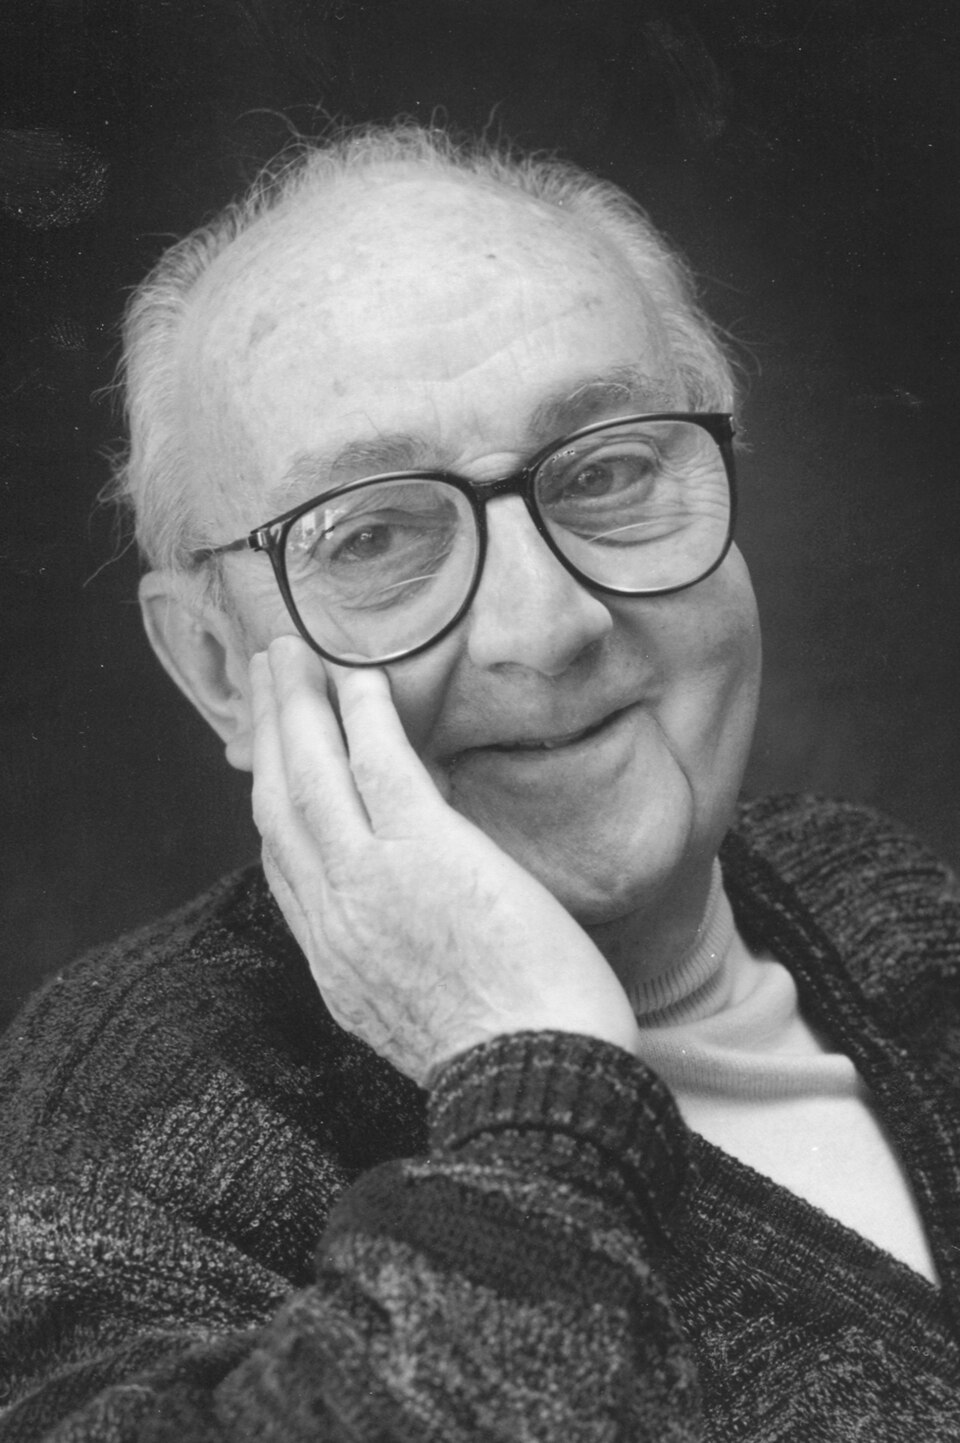
\includegraphics[height=0.42\textheight]{ch0_box.jpg}\\[1mm]
\imgcap{George E. P. Box (1919--2013)}
\imgcredit{https://commons.wikimedia.org/wiki/File:GeorgeEPBox_(cropped).jpg}{Foto: DavidMCEddy (2011); CC BY-SA 3.0; Wikimedia Commons}
\end{column}
\end{columns}
\end{frame}

\begin{frame}{Pasul 1: datele}
\itemsize{\footnotesize}
\begin{center}
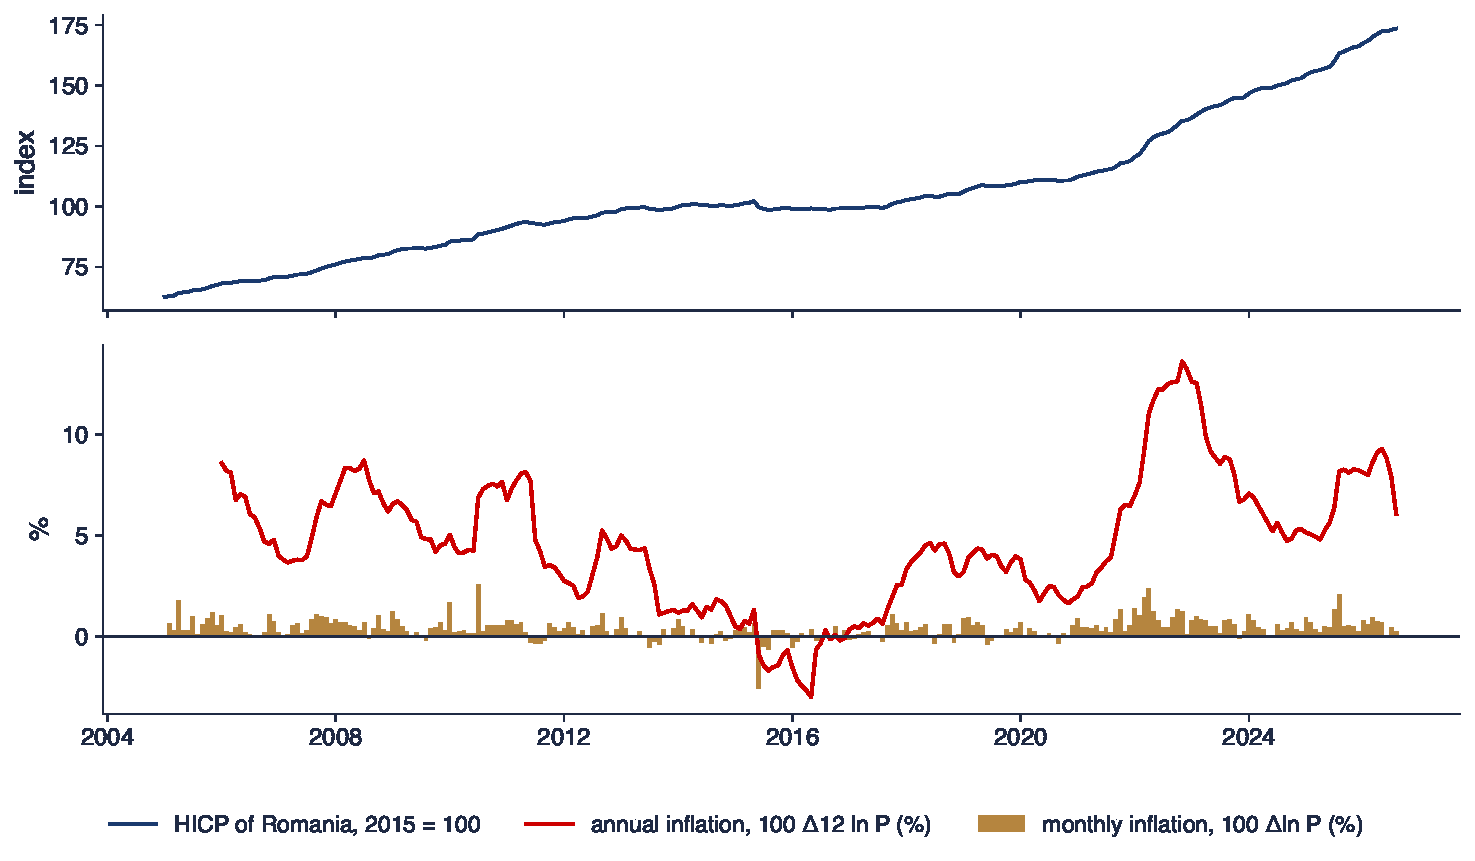
\includegraphics[width=0.97\textwidth,height=0.6\textheight,keepaspectratio]{tsa_ch15_bj_data.pdf}
\end{center}
\vspace{-0.25cm}
\begin{itemize}
    \item Sus: IAPC, 2015 = 100; jos: inflația lunară $100\Delta\ln P_t$ (bare) și inflația anuală $100\Delta_{12}\ln P_t$ (linie)
\end{itemize}
\quantlet{TSA\_ch15\_box\_jenkins}{\qlurl{TSA_ch15_box_jenkins}}
\end{frame}

\begin{frame}{Interpretarea datelor}
\itemsize{\small}
\begin{itemize}
    \item \textbf{Trend}: indicele crește aproape în fiecare lună; logaritmul este scala firească
    \begin{itemize}
        \item inflația lunară are media 0{,}39\%; inflația anuală variază între $\ensuremath{-}3{,}0\%$ (mai 2016) și 13{,}6\% (noiembrie 2022)
    \end{itemize}
    \item \textbf{Sezonalitatea}: ianuarie are în medie 0{,}74\%, iunie $\ensuremath{-}0{,}03\%$ (alimentele proaspete)
    \begin{itemize}
        \item un tipar sezonier în $\Delta\ln P_t$: vom avea nevoie de $\Delta_{12}$ sau de termeni sezonieri
    \end{itemize}
    \item \textbf{Șocurile}: modificările de taxe mută prețurile într-o singură lună
    \begin{itemize}
        \item iulie--august 2025: încetarea plafonării prețului la electricitate și creșterea TVA; inflația anuală de la 6{,}4\% la 8{,}2\%
    \end{itemize}
\end{itemize}
\end{frame}

\begin{frame}{Pasul 2: teste de rădăcină unitară și de staționaritate}
\itemsize{\footnotesize}
\begin{center}
\footnotesize
\begin{tabular}{lccccc}
\toprule
\textbf{Seria} & \textbf{Termeni} & ADF $\tau$ & $p$ & KPSS $\eta$ (5\%: val. critică) & \textbf{Verdict} \\
\midrule
$100\ln P_t$ & const., trend & $\ensuremath{-}0{,}96$ & 0{,}949 & 0{,}314 (0{,}146) & rădăcină unitară \\
$\Delta\ln P_t$ & const. & $\ensuremath{-}4{,}00$ & 0{,}001 & 0{,}431 (0{,}463) & staționară, sezonieră \\
$\Delta_{12}\ln P_t$ & const. & $\ensuremath{-}1{,}69$ & 0{,}435 & 0{,}424 (0{,}463) & neconcludent \\
$z_t = \Delta\Delta_{12}\ln P_t$ & const. & $\ensuremath{-}4{,}83$ & $<$\,0{,}001 & 0{,}113 (0{,}463) & staționară \\
\bottomrule
\end{tabular}
\end{center}
\begin{itemize}
    \item ADF: $H_0$ rădăcină unitară, decalaje după AIC \refDF; KPSS: $H_0$ staționaritate \refKPSS; valorile critice ADF la 5\%: $\ensuremath{-}3{,}43$ (cu trend), $\ensuremath{-}2{,}87$ (cu constantă)
    \item Inflația anuală: nici ADF, nici KPSS nu respinge: un rezultat neconcludent, ca în \tsachlink{https://danpele.github.io/Time-Series-Analysis/RO/Cursuri/capitol3_radacini_unitare_modele_arima.pdf}{Capitolul 3}
    \item Decizia: $d = 1$, $D = 1$: modelăm $z_t$, iar ambele teste arată că este staționară
\end{itemize}\quantlet{TSA\_ch15\_box\_jenkins}{\qlurl{TSA_ch15_box_jenkins}}
\end{frame}

\begin{frame}{Pasul 3: identificarea din corelograma lui $z_t$}
\itemsize{\footnotesize}
\begin{center}
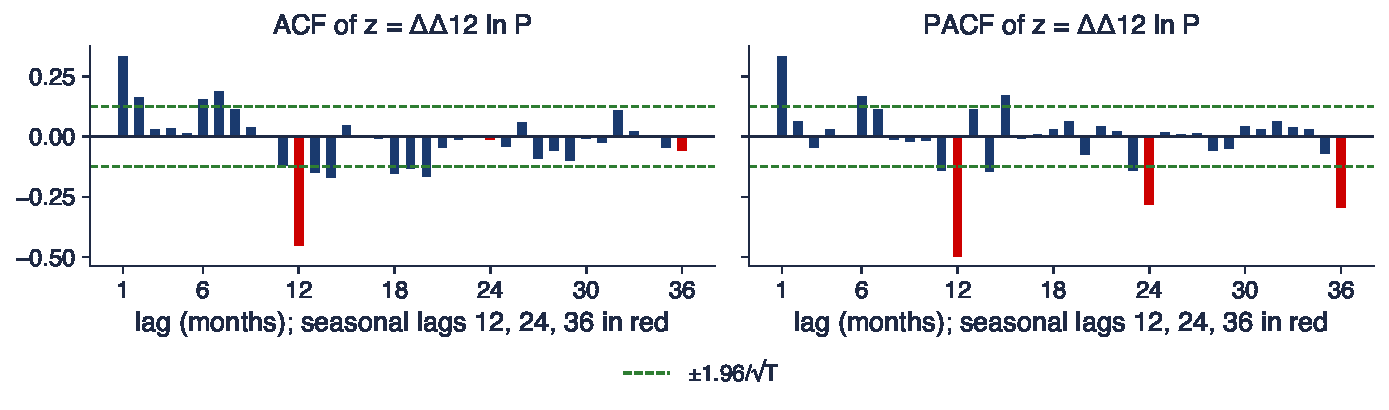
\includegraphics[width=0.97\textwidth,height=0.55\textheight,keepaspectratio]{tsa_ch15_bj_acf.pdf}
\end{center}
\vspace{-0.25cm}
\begin{itemize}
    \item ACF și PACF pentru $z_t = \Delta\Delta_{12}\ln P_t$, decalajele 1--36, $T = 247$; decalajele sezoniere în roșu; banda $\pm 0{,}125$
\end{itemize}
\quantlet{TSA\_ch15\_box\_jenkins}{\qlurl{TSA_ch15_box_jenkins}}
\end{frame}

\begin{frame}{Interpretarea corelogramei}
\itemsize{\small}
\begin{itemize}
    \item \textbf{Partea obișnuită}: $\hat\rho_1 = 0{,}33$, $\hat\rho_2 = 0{,}16$; PACF $\hat\phi_{11} = 0{,}33$, apoi mici: un AR(1)
    \begin{itemize}
        \item este posibil și un MA(1): ACF și PACF scad amîndouă după decalajul 1
    \end{itemize}
    \item \textbf{Partea sezonieră}: ACF $\ensuremath{-}0{,}45$ la decalajul 12, apoi $\ensuremath{-}0{,}01$ la 24; PACF $\ensuremath{-}0{,}50$, $\ensuremath{-}0{,}28$, $\ensuremath{-}0{,}29$ la 12, 24, 36
    \begin{itemize}
        \item o singură valoare sezonieră mare în ACF și o PACF sezonieră care descrește: un MA(1) sezonier
    \end{itemize}
    \item Primul candidat: SARIMA$(1,1,0)(0,1,1)_{12}$ pentru $\ln P_t$; sateliții de la decalajele 11 și 13 sînt produsul $\rho_1\rho_{12}$
\end{itemize}
\end{frame}

\begin{frame}{Pasul 4: estimarea candidaților}
\itemsize{\footnotesize}
\begin{center}
\footnotesize
\begin{tabular}{lccccc}
\toprule
\textbf{Modelul} & param. & AICc & BIC & LB(12) $p$ & LB(24) $p$ \\
\midrule
$(1,1,0)(0,1,1)_{12}$, identificat & 3 & 295{,}2 & 305{,}3 & 0{,}004 & 0{,}004 \\
${(1,1,1)(0,1,1)}_{12}$ & 4 & 285{,}4 & 298{,}9 & 0{,}029 & 0{,}088 \\
${(2,1,1)(0,1,1)}_{12}$ & 5 & 282{,}6 & 299{,}4 & 0{,}233 & 0{,}237 \\
${(1,1,2)(0,1,1)}_{12}$ & 5 & 282{,}8 & 299{,}6 & 0{,}233 & 0{,}217 \\
${(1,1,1)(1,1,1)}_{12}$ & 5 & 287{,}7 & 304{,}5 & 0{,}017 & 0{,}070 \\
\bottomrule
\end{tabular}
\end{center}
\begin{itemize}
    \item Toate cele 36 de modele SARIMA$(p,1,q)(P,1,Q)_{12}$ cu $p, q \le 2$, $P, Q \le 1$, pe eșantionul de antrenare pînă în august 2024 ($T = 236$); ordonate după BIC
    \item param.: toți parametrii estimați, inclusiv varianța; Ljung--Box pe reziduuri cu $m - k$ grade de libertate, $k$ = parametrii ARMA
    \item Modelul identificat nu trece verificarea reziduurilor; cel mai mic BIC, $(1,1,1)(0,1,1)$, eșuează la decalajul 12; modelul ales este $(2,1,1)(0,1,1)_{12}$, cel mai mic BIC dintre modelele care trec
\end{itemize}\quantlet{TSA\_ch15\_box\_jenkins}{\qlurl{TSA_ch15_box_jenkins}}
\end{frame}

\begin{frame}{Pasul 4: modelul ales}
\itemsize{\footnotesize}
\begin{center}
\footnotesize
\begin{tabular}{lcccc}
\toprule
\textbf{Parametrul} & \textbf{Estimarea} & SE & $z$ & $p$ \\
\midrule
$\phi_1$ (ar.L1) & $1{,}156$ & $0{,}149$ & $7{,}76$ & $<$\,0{,}001 \\
$\phi_2$ (ar.L2) & $\ensuremath{-}0{,}183$ & $0{,}122$ & $\ensuremath{-}1{,}50$ & 0{,}133 \\
$\theta_1$ (ma.L1) & $\ensuremath{-}0{,}856$ & $0{,}099$ & $\ensuremath{-}8{,}61$ & $<$\,0{,}001 \\
$\Theta_1$ (ma.S.L12) & $\ensuremath{-}0{,}935$ & $0{,}098$ & $\ensuremath{-}9{,}55$ & $<$\,0{,}001 \\
$\sigma^2$ & $0{,}179$ & & & \\
\bottomrule
\end{tabular}
\end{center}
\begin{itemize}
    \item $(1 - \phi_1L - \phi_2L^2)\,z_t = (1 + \theta_1L)(1 + \Theta_1L^{12})\,\varepsilon_t$, $z_t = \Delta\Delta_{12}\,100\ln P_t$
    \item $\hat\Theta_1$ aproape de $-1$: tiparul sezonier este aproape fix, iar $\Delta_{12}$ aproape se anulează; variabilele dummy sezoniere ar fi o alternativă
    \item Cea mai mică rădăcină AR are modulul 1{,}034: șocurile inflației sînt foarte persistente, ca în \tsachlink{https://danpele.github.io/Time-Series-Analysis/RO/Cursuri/capitol2_modele_arma.pdf}{Capitolele 2} și \tsachlink{https://danpele.github.io/Time-Series-Analysis/RO/Cursuri/capitol8_memorie_lunga_arfima.pdf}{8}
\end{itemize}\quantlet{TSA\_ch15\_box\_jenkins}{\qlurl{TSA_ch15_box_jenkins}}
\end{frame}

\begin{frame}{Pasul 5: verificarea reziduurilor}
\itemsize{\footnotesize}
\begin{center}
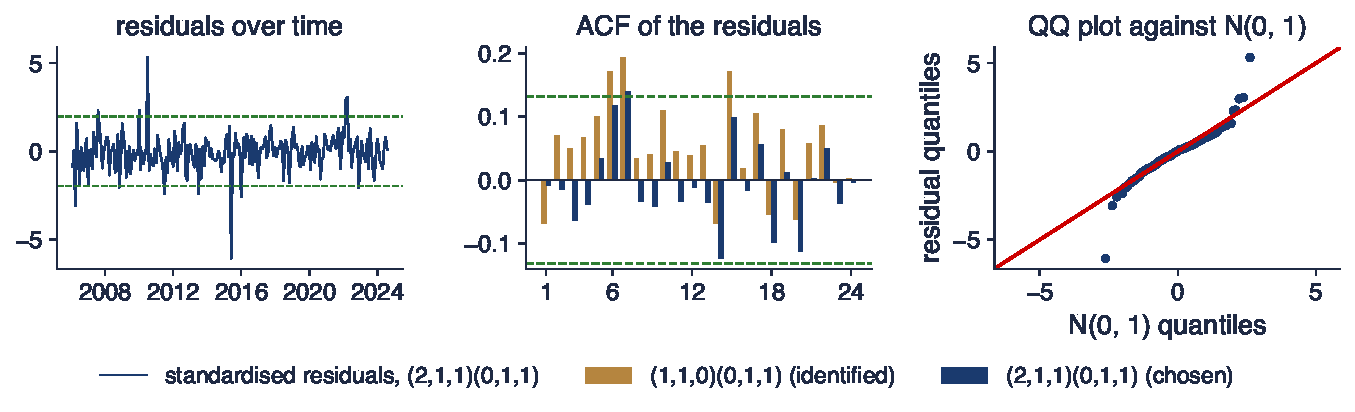
\includegraphics[width=0.97\textwidth,height=0.55\textheight,keepaspectratio]{tsa_ch15_bj_diag.pdf}
\end{center}
\vspace{-0.25cm}
\begin{itemize}
    \item Reziduurile standardizate ale modelului ales; ACF a reziduurilor ambelor modele; QQ plot față de $N(0, 1)$
\end{itemize}
\quantlet{TSA\_ch15\_box\_jenkins}{\qlurl{TSA_ch15_box_jenkins}}
\end{frame}

\begin{frame}{Interpretarea verificării reziduurilor}
\itemsize{\small}
\begin{itemize}
    \item \textbf{Nu mai rămîne autocorelație}: Ljung--Box $Q(12) = 10{,}49$ ($8$ grade de libertate, $p = 0{,}233$), $Q(24) = 24{,}13$ ($p = 0{,}237$)
    \begin{itemize}
        \item modelul identificat avea $p = 0{,}004$ și 0{,}004: termenii AR și MA în plus reduc autocorelația de la decalajele 6--7
    \end{itemize}
    \item \textbf{Nu este Normal}: Jarque--Bera 450, coeficientul de boltire 9{,}9
    \begin{itemize}
        \item cele mai mari două reziduuri: iunie 2015 ($\ensuremath{-}6{,}1\sigma$, reducerea TVA la alimente) și iulie 2010 ($5{,}3\sigma$, creșterea TVA)
    \end{itemize}
    \item Consecința: prognozele punctuale sînt bune, dar intervalele Normale sînt prea înguste cînd se schimbă taxele; variabile dummy pentru modificările de taxe cunoscute ar ajuta
\end{itemize}
\end{frame}

\begin{frame}{Pasul 6: prognoze}
\itemsize{\footnotesize}
\begin{center}
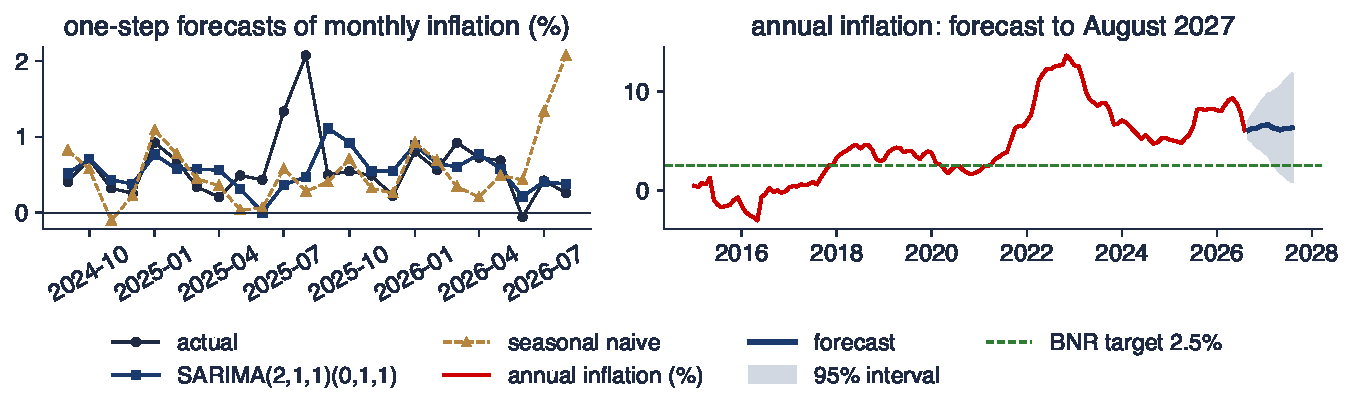
\includegraphics[width=0.97\textwidth,height=0.55\textheight,keepaspectratio]{tsa_ch15_bj_forecast.pdf}
\end{center}
\vspace{-0.25cm}
\begin{itemize}
    \item Stînga: prognoze pe un pas ale inflației lunare pe eșantionul de test (septembrie 2024 -- august 2026), cu parametrii estimați pe eșantionul de antrenare; dreapta: prognoze ale inflației anuale pînă în august 2027, cu intervale de 95\%, modelul reestimat pe toate datele
\end{itemize}
\quantlet{TSA\_ch15\_box\_jenkins}{\qlurl{TSA_ch15_box_jenkins}}
\end{frame}

\begin{frame}{Interpretarea prognozelor}
\itemsize{\footnotesize}
\begin{center}
\footnotesize
\begin{tabular}{lccc}
\toprule
\textbf{Inflația lunară, eșantion de test} & RMSE & MAE & MASE \\
\midrule
SARIMA$(2,1,1)(0,1,1)_{12}$ & 0{,}45 & 0{,}28 & 0{,}66 \\
naiv sezonier & 0{,}64 & 0{,}42 & 0{,}99 \\
naiv & 0{,}51 & 0{,}38 & 0{,}88 \\
\bottomrule
\end{tabular}
\end{center}
\begin{itemize}
    \item SARIMA are cele mai mici erori, dar testul Diebold--Mariano (HLN) nu respinge acuratețea egală: $\ensuremath{-}1{,}40$ ($p = 0{,}174$) față de naivul sezonier, $\ensuremath{-}0{,}47$ ($p = 0{,}642$) față de metoda naivă
    \begin{itemize}
        \item 24 de luni sînt puține; cele mai mari erori: august 2025 (2{,}07\%, față de 0{,}47\%) și iulie 2025 (1{,}34\%, față de 0{,}37\%): decizii privind taxele și energia pe care niciun model univariat nu le poate anticipa
    \end{itemize}
    \item Inflația anuală: 6{,}1\% în august 2026; prognoza 6{,}1\% pentru septembrie 2026 [5{,}3; 6{,}9], 6{,}3\% pentru august 2027 [0{,}9; 11{,}8]
    \begin{itemize}
        \item saltul TVA din august 2025 iese din fereastra de 12 luni în august 2026; intervalul la 12 luni este larg: o rădăcină aproape unitară în $\Delta\ln P_t$
    \end{itemize}
\end{itemize}\quantlet{TSA\_ch15\_box\_jenkins}{\qlurl{TSA_ch15_box_jenkins}}
\end{frame}

\begin{frame}{Recapitulare: Box--Jenkins pe inflația din România}
\itemsize{\small}
\begin{itemize}
    \item Grafic, transformare, testare: $\ln P_t$ are nevoie de $d = 1$ și $D = 1$
    \item Corelograma sugerează $(1,1,0)(0,1,1)_{12}$; verificarea reziduurilor îl respinge; modelul ales este $(2,1,1)(0,1,1)_{12}$
    \item În afara eșantionului, cîștigul față de metoda naivă sezonieră nu este semnificativ; șocurile fiscale domină erorile
\end{itemize}
\end{frame}


%=============================================================================
\section{Examenul}
%=============================================================================

\begin{frame}{Examenul scris: formatul}
\itemsize{\small}
\begin{columns}[T]
\begin{column}{0.58\textwidth}
\begin{itemize}
    \item \textbf{70\% din nota finală}; scris, 2 ore
    \begin{itemize}
        \item cinci subiecte, toate obligatorii; 9 puncte pentru subiecte plus 1 punct din oficiu
    \end{itemize}
    \item \textbf{Trei tipuri de subiecte}
    \begin{itemize}
        \item o derivare scurtă: momente, staționaritate, ACF sau forma unui proces
        \item interpretarea rezultatelor obținute cu software: estimări, teste, corelograme, tabele VAR și VECM
        \item alegerea modelului și o prognoză calculată de mînă din rezultate
    \end{itemize}
    \item Valorile critice necesare sînt tipărite în rezultate, ca în problemele de mai jos
\end{itemize}
\end{column}
\begin{column}{0.38\textwidth}
\centering
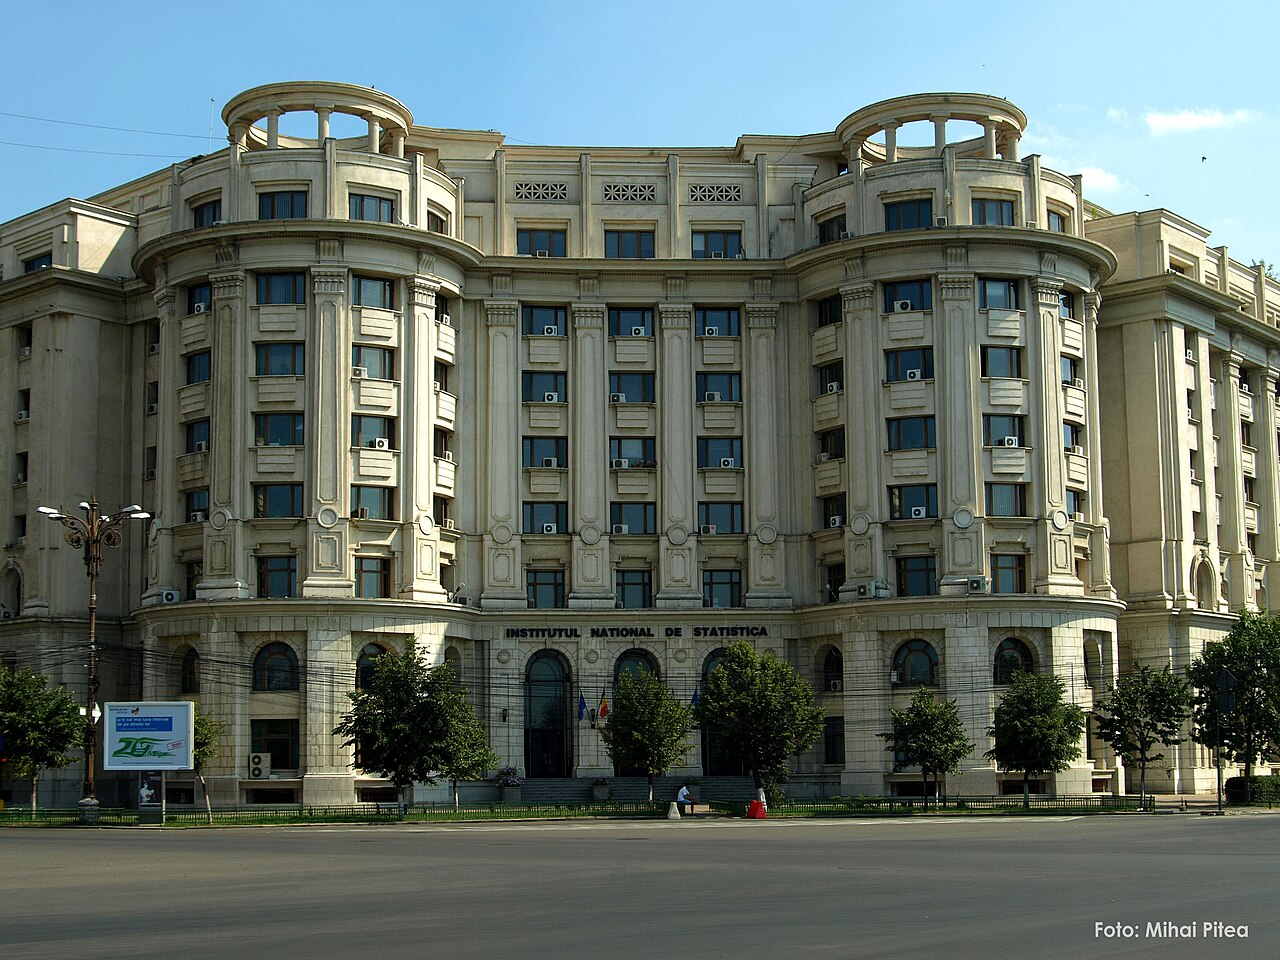
\includegraphics[height=0.40\textheight]{ch2_ins_bucharest_2009.jpg}\\[1mm]
\imgcap{Institutul Național de Statistică, București: sursa multor serii de examen}
\imgcredit{https://commons.wikimedia.org/wiki/File:Institutul_Na\%C8\%9Bional_de_Statistic\%C4\%83.jpg}{Foto: Dan Mihai Pitea (2009); CC BY-SA 3.0; Wikimedia Commons}
\end{column}
\end{columns}
\end{frame}

\begin{frame}{Conținutul evaluat}
\itemsize{\small}
\begin{itemize}
    \item \textbf{\tsachlink{https://danpele.github.io/Time-Series-Analysis/RO/Cursuri/capitol0_introducere.pdf}{Capitolele 0}--\tsachlink{https://danpele.github.io/Time-Series-Analysis/RO/Cursuri/capitol10_spatiul_starilor_kalman_markov_switching.pdf}{10}}: cursuri și seminarii
    \begin{itemize}
        \item definițiile și formulele de pe slide-urile „Noțiuni necesare azi” ale fiecărui seminar
        \item calculele din Partea A a seminariilor, pe hîrtie
    \end{itemize}
    \item \textbf{Citirea rezultatelor}: tabele ca în Partea B și ca în acest capitol
    \begin{itemize}
        \item rezultate EViews sau Python: aceleași cifre sub alte nume (AR(1), ar.L1; SAR(12), ar.S.L12)
        \item la examen nu se scrie cod
    \end{itemize}
    \item \textbf{Ponderea principală}: ARIMA și SARIMA, rădăcini unitare, VAR și cauzalitate Granger, cointegrare și VECM, GARCH
    \begin{itemize}
        \item \tsachlink{https://danpele.github.io/Time-Series-Analysis/RO/Cursuri/capitol11_foundation_models_serii_timp.pdf}{Capitolele 11}--\tsachlink{https://danpele.github.io/Time-Series-Analysis/RO/Cursuri/capitol14_modele_garch_multivariate.pdf}{14} sînt pentru studiu individual (nu se examinează, dacă titularul nu decide altfel)
    \end{itemize}
\end{itemize}
\end{frame}

\begin{frame}{Criterii de notare}
\itemsize{\small}
\begin{itemize}
    \item \textbf{Metoda}: formula sau ecuația, cu cifrele înlocuite
    \begin{itemize}
        \item o metodă corectă cu o greșeală de calcul primește cea mai mare parte a punctajului
    \end{itemize}
    \item \textbf{Rezultatul}: cifra, cu unitatea de măsură (\%, puncte procentuale, luni) și semnul ei
    \begin{itemize}
        \item pentru un test: $H_0$, statistica, valoarea critică sau $p$-valoarea, decizia
    \end{itemize}
    \item \textbf{Interpretarea}: trei pînă la cinci fraze, statistice și economice
    \begin{itemize}
        \item o cifră corectă cu o interpretare greșită nu primește tot punctajul
        \item precizați ce nu poate arăta modelul (cauzalitatea, rupturile structurale, viitorul politicilor)
    \end{itemize}
\end{itemize}
\end{frame}

\begin{frame}{Tipuri de probleme}
\itemsize{\small}
\begin{center}
\footnotesize
\begin{tabular}{>{\raggedright\arraybackslash}p{4.6cm}>{\raggedright\arraybackslash}p{1.4cm}>{\raggedright\arraybackslash}p{5.2cm}}
\toprule
\textbf{Tipul} & \textbf{Capitole} & \textbf{Exemplu în acest capitol} \\
\midrule
derivare: momente, staționaritate, diferențiere & 1--3 & Problema 1: trend plus erori AR(1) \\
corelogramă și test de rădăcină unitară: identificare & 1--3 & Problema 2: PIB-ul României \\
rezultate SARIMA și o prognoză de mînă & 2--4 & Problema 3: inflația din România \\
rezultate VAR și Granger & 6 & Problema 4: creștere, inflație, ROBOR \\
rezultate de cointegrare și VECM & 7 & Problema 5: randamentele SUA \\
rezultate GARCH și VaR 1\% & 5 & Problema 6: BET \\
evaluarea prognozelor; spațiul stărilor și regimuri & 4, 8--10 & Problemele 7 și 8 \\
\bottomrule
\end{tabular}
\end{center}
\begin{itemize}
    \item Cele opt probleme de mai jos sînt exemple de recapitulare, cu rezolvări complete; examenul are subiecte proprii
\end{itemize}
\end{frame}

\begin{frame}{Problema 1: un trend cu erori AR(1)}
\itemsize{\footnotesize}
\begin{itemize}
    \item \textbf{Context}
    \begin{itemize}
        \item $Y_t = 10 + 0{,}5t + u_t$, $u_t = 0{,}6u_{t-1} + \varepsilon_t$, $\varepsilon_t \sim WN(0, 1)$
        \item La $T = 100$ observăm $Y_T = 62$
    \end{itemize}
    \item \textbf{Cerințe}
\begin{enumerate}
    \item Calculați $E(Y_t)$ și $\mathrm{Var}(Y_t)$ și precizați dacă $Y_t$ este staționar.
    \item Arătați că $\Delta Y_t$ este un ARMA(1,1) cu $\theta = -1$ și calculați $\rho_{\Delta Y}(1)$.
    \item Prognozați $Y_{T+1}$ și $Y_{T+10}$ cu modelul corect și dați varianța erorii pe 10 pași.
    \item Explicați ce nu este în regulă dacă analistul diferențiază $Y_t$.
\end{enumerate}
\end{itemize}
\end{frame}

\begin{frame}{Problema 1: rezolvare}
\itemsize{\footnotesize}
\begin{enumerate}
    \item $E(Y_t) = 10 + 0{,}5t$ depinde de $t$: nestaționar; $\mathrm{Var}(Y_t) = 1/(1 - 0{,}36) = 1{,}5625$ este constantă: \textbf{staționar în jurul trendului}
    \item $\Delta Y_t = 0{,}5 + \Delta u_t$ și $(1 - 0{,}6L)\Delta u_t = (1 - L)\varepsilon_t$: ARMA(1,1), $\theta = -1$; $\gamma(0) = 1{,}25$, $\gamma(1) = \ensuremath{-}0{,}25$, $\rho(1) = \ensuremath{-}0{,}20$
    \item $u_T = 62 - 10 - 50 = 2{,}0$; $\hat Y_{T+1} = 10 + 50{,}5 + 0{,}6 \cdot 2 = 61{,}70$; $\hat Y_{T+10} = 10 + 55 + 0{,}6^{10} \cdot 2 = 65{,}01$; varianța $(1 - 0{,}6^{20})/(1 - 0{,}36) = 1{,}562$
    \item Rădăcina MA este 1: $\Delta Y_t$ nu este invertibil; $\hat\rho_1 < 0$ și un coeficient MA aproape de $-1$ sînt semnele supradiferențierii
\end{enumerate}
\begin{itemize}
    \item \textbf{Interpretare}
    \begin{itemize}
        \item Un șoc se stinge: după 10 perioade mai rămîne doar $0{,}012$ din abatere, iar varianța erorii rămîne mărginită
        \item Tratamentul urmează tipul trendului: eliminăm trendul dintr-o serie staționară în jurul trendului, diferențiem o serie cu rădăcină unitară (\tsachlink{https://danpele.github.io/Time-Series-Analysis/RO/Cursuri/capitol3_radacini_unitare_modele_arima.pdf}{Capitolul 3})
    \end{itemize}
\end{itemize}
\end{frame}

\begin{frame}{Problema 2: identificarea PIB-ului României}
\itemsize{\footnotesize}
\begin{center}
\scriptsize
\begin{tabular}{lcccccc}
\toprule
\textbf{Seria} & Termeni & ADF $\tau$ & $p$ & val. critice 1\%; 5\%; 10\% & KPSS & val. critică 5\% \\
\midrule
$100\ln Y_t$ & c, t & $\ensuremath{-}2{,}31$ & 0{,}428 & $\ensuremath{-}4{,}05$; $\ensuremath{-}3{,}45$; $\ensuremath{-}3{,}15$ & 0{,}198 & 0{,}146 \\
$100\Delta\ln Y_t$ & c & $\ensuremath{-}10{,}77$ & $<$\,0{,}001 & $\ensuremath{-}3{,}49$; $\ensuremath{-}2{,}89$; $\ensuremath{-}2{,}58$ & 0{,}263 & 0{,}463 \\
\bottomrule
\end{tabular}
\end{center}
\begin{itemize}
    \item \textbf{Context}
    \begin{itemize}
        \item PIB-ul real al României, ajustat sezonier (Eurostat), 2000Q1 -- 2026Q2
        \item Creșterea $g_t = 100\Delta\ln Y_t$: ACF $\ensuremath{-}0{,}05$; $\ensuremath{-}0{,}14$; PACF $\ensuremath{-}0{,}05$; $\ensuremath{-}0{,}14$ (decalajele 1, 2; banda $\pm 0{,}19$); Ljung--Box $Q(8) = 7{,}28$, $p = 0{,}506$; $\chi^2_{0,95}(8) = 15{,}51$
    \end{itemize}
    \item \textbf{Cerințe}
\begin{enumerate}
    \item Descrieți testul ADF și decideți dacă $\ln Y_t$ și $g_t$ sînt staționare.
    \item Precizați dacă testul KPSS confirmă rezultatul.
    \item Identificați procesul cu metoda Box--Jenkins.
    \item Deriva estimată este $0{,}81$ (SE $0{,}30$): scrieți modelul și interpretați deriva.
\end{enumerate}
\end{itemize}
\end{frame}

\begin{frame}{Problema 2: rezolvare}
\itemsize{\footnotesize}
\begin{enumerate}
    \item ADF: $\Delta y_t = c + bt + \gamma y_{t-1} + \sum\delta_j\Delta y_{t-j} + \varepsilon_t$, $H_0$: $\gamma = 0$ (rădăcină unitară); $\ln Y_t$: $\ensuremath{-}2{,}31 > \ensuremath{-}3{,}45$: nu se respinge; $g_t$: $\ensuremath{-}10{,}77 < \ensuremath{-}3{,}49$: se respinge
    \item KPSS ($H_0$: staționaritate): $0{,}198 > 0{,}146$ respinge pentru nivel, $0{,}263 < 0{,}463$ nu respinge pentru creștere: $\ln Y_t \sim I(1)$
    \item ACF și PACF ale lui $g_t$ sînt în bandă, $Q(8) = 7{,}28 < 15{,}51$: creșterea este zgomot alb în jurul mediei
    \item ARIMA(0,1,0) cu derivă: $100\ln Y_t = 100\ln Y_{t-1} + 0{,}81 + \varepsilon_t$, $\hat\sigma = 2{,}47$; $t = 2{,}72$
\end{enumerate}
\begin{itemize}
    \item \textbf{Interpretare}
    \begin{itemize}
        \item Economia crește cu circa 0{,}81\% pe trimestru, adică aproximativ 3{,}2\% pe an; surprizele trimestriale nu sînt previzibile
        \item Un șoc asupra nivelului este permanent: recesiunile din 2009 și 2020 au mutat definitiv traiectoria PIB-ului
    \end{itemize}
\end{itemize}
\end{frame}

\begin{frame}{Problema 3: rezultate SARIMA și o prognoză de mînă}
\itemsize{\footnotesize}
\begin{center}
\scriptsize
\begin{tabular}{lcccc}
\toprule
\textbf{Variabila dependentă: $z_t$} & Coeficient & SE & $z$ & $p$ \\
\midrule
AR(1) & $0{,}353$ & $0{,}054$ & $6{,}53$ & $<$\,0{,}001 \\
SAR(12) & $\ensuremath{-}0{,}488$ & $0{,}035$ & $\ensuremath{-}13{,}90$ & $<$\,0{,}001 \\
SIGMASQ & $0{,}254$ & & & \\
Ljung--Box $Q(12)$ & $22{,}64$ & & & 0{,}012 \\
\bottomrule
\end{tabular}
\end{center}
\begin{itemize}
    \item \textbf{Context}
    \begin{itemize}
        \item $z_t = \Delta\Delta_{12}\,100\ln \mathrm{IAPC}_t$ („DLOG(IPC,1,12)”), România, februarie 2006 -- august 2026, $T = 247$
        \item Ultimele valori: $z$ = $\ensuremath{-}1{,}814$ (august 2026), $0{,}090$ (septembrie 2025), $1{,}794$ (august 2025); inflația anuală în august 2026: 6{,}085\%
    \end{itemize}
    \item \textbf{Cerințe}
\begin{enumerate}
    \item Scrieți ecuația modelului și interpretați coeficienții.
    \item Testați dacă reziduurile sînt zgomot alb.
    \item Prognozați $z$ și rata anuală a inflației pentru septembrie 2026.
\end{enumerate}
\end{itemize}
\end{frame}

\begin{frame}{Problema 3: rezolvare}
\itemsize{\scriptsize}
\begin{enumerate}
    \item $(1 - \phi L)(1 - \Phi L^{12})z_t = \varepsilon_t$, deci $z_t = \phi z_{t-1} + \Phi z_{t-12} - \phi\Phi z_{t-13} + \varepsilon_t$
    \item $\hat\phi = 0{,}353$: o surpriză lunară continuă și luna următoare; $\hat\Phi = \ensuremath{-}0{,}488 < 0$: o surpriză dintr-o lună se inversează parțial în aceeași lună a anului următor; ambele semnificative; rădăcinile AR inversate 0{,}35 și 0{,}94 $< 1$: staționar
    \item Ljung--Box $Q(12) = 22{,}64$ cu $12 - 2 = 10$ grade de libertate, $p = 0{,}012$: ipoteza de zgomot alb se respinge la 5\%; modelul lasă o parte din autocorelație (comparați cu Pasul 5 de mai sus)
    \item $\hat z_{T+1} = 0{,}353(\ensuremath{-}1{,}814) + (\ensuremath{-}0{,}488)(0{,}090) - (\ensuremath{-}0{,}173)(1{,}794) = \ensuremath{-}0{,}641 + (\ensuremath{-}0{,}044) + 0{,}310 = \ensuremath{-}0{,}375$
    \item Inflația anuală: $\Delta_{12}\ln P_{T+1} = \Delta_{12}\ln P_T + z_{T+1} = 6{,}085 + (\ensuremath{-}0{,}375) = 5{,}71\%$
\end{enumerate}
\begin{itemize}
    \item \textbf{Interpretare}
    \begin{itemize}
        \item Se așteaptă ca inflația să scadă în continuare în septembrie 2026, pe măsură ce șocul fiscal de anul trecut iese din fereastra de 12 luni
        \item Autocorelația reziduală: un model mai bogat (ca la Pasul 4) ar schimba puțin prognoza; un interval de 95\% are nevoie de $\hat\sigma$
    \end{itemize}
\end{itemize}
\end{frame}

\begin{frame}{Problema 4: rezultate VAR și cauzalitate Granger}
\itemsize{\scriptsize}
\begin{center}
\scriptsize
\begin{tabular}{lccc}
\toprule
\textbf{Ecuația ROBOR} & coef. [$t$] & & coef. [$t$] \\
\midrule
$g_{t-1}$ & $0{,}142$ [$3{,}49$] & $g_{t-2}$ & $0{,}074$ [$1{,}73$] \\
$\pi_{t-1}$ & $0{,}240$ [$2{,}78$] & $\pi_{t-2}$ & $\ensuremath{-}0{,}172$ [$\ensuremath{-}1{,}89$] \\
$i_{t-1}$ & $1{,}042$ [$10{,}16$] & $i_{t-2}$ & $\ensuremath{-}0{,}119$ [$\ensuremath{-}1{,}20$] \\
constanta & $\ensuremath{-}0{,}109$ [$\ensuremath{-}0{,}55$] & $R^2$ & 0{,}93 \\
\bottomrule
\end{tabular}
\end{center}
\begin{center}
\scriptsize
\begin{tabular}{lcc}
\toprule
\textbf{Ipoteza nulă} & $F$ & $p$ \\
\midrule
$g$ nu cauzează Granger $i$ & 7{,}26 & 0{,}001 \\
$\pi$ nu cauzează Granger $i$ & 4{,}74 & 0{,}011 \\
$i$ nu cauzează Granger $\pi$ & 0{,}89 & 0{,}417 \\
\bottomrule
\end{tabular}
\end{center}
\begin{itemize}
    \item \textbf{Context}
    \begin{itemize}
        \item VAR(2) pentru România, T3 2005 -- T2 2026 ($T = 84$): creșterea PIB $g$, inflația anuală $\pi$, ROBOR 3M $i$
    \end{itemize}
    \item \textbf{Cerințe}
\begin{enumerate}
    \item Descrieți cauzalitatea Granger și interpretați tabelul.
    \item Scrieți ecuația ROBOR și cuantificați efectul pe termen lung al unei creșteri permanente a inflației cu 1 pp asupra ROBOR.
    \item Recalculați primul $F$ din $RSS_R = 69{,}27$ și $RSS_U = 58{,}27$.
\end{enumerate}
\end{itemize}
\end{frame}

\begin{frame}{Problema 4: rezolvare}
\itemsize{\scriptsize}
\begin{enumerate}
    \item $x$ cauzează Granger $y$ dacă decalajele lui $x$ îmbunătățesc prognoza lui $y$, dată fiind istoria lui $y$ (test $F$ comun) \refGranger; creșterea și inflația ajută la prognoza ROBOR ($p =$ 0{,}001 și 0{,}011); ROBOR nu ajută la prognoza inflației ($p = 0{,}417$)
    \item $i_t = \ensuremath{-}0{,}109 + 0{,}142g_{t-1} + 0{,}074g_{t-2} + 0{,}240\pi_{t-1} + (\ensuremath{-}0{,}172)\pi_{t-2} + 1{,}042i_{t-1} + (\ensuremath{-}0{,}119)i_{t-2} + u_t$
    \item Pe termen lung ($i_t = i_{t-1}$, $\pi_t = \pi_{t-1}$): $\partial i/\partial\pi = (0{,}240 + (\ensuremath{-}0{,}172))/(1 - 1{,}042 - (\ensuremath{-}0{,}119)) = 0{,}068/0{,}076 = 0{,}90$ pp
    \item $F = \frac{(69{,}27 - 58{,}27)/2}{58{,}27/77} = 7{,}26 > F_{0,95}(2, 77) = 3{,}12$: $H_0$ se respinge
\end{enumerate}
\begin{itemize}
    \item \textbf{Interpretare}
    \begin{itemize}
        \item Dobînda interbancară urmează economia și inflația, așa cum ar implica reacția unei bănci centrale; legătura inversă nu se vede în datele trimestriale
        \item Efectul pe termen lung împarte la $0{,}076$, un număr apropiat de zero: este imprecis; cauzalitatea Granger înseamnă predictibilitate, nu dovada unui efect de politică
    \end{itemize}
\end{itemize}
\end{frame}

\begin{frame}{Problema 5: rezultate de cointegrare și VECM}
\itemsize{\scriptsize}
\begin{center}
\scriptsize
\begin{tabular}{lcccc}
\toprule
\textbf{Testul urmei Johansen} & $r = 0$ & $r \le 1$ & $r \le 2$ & \\
\midrule
statistica & 54{,}60 & 21{,}57 & 3{,}12 & \\
valoarea critică 5\% & 29{,}80 & 15{,}49 & 3{,}84 & \\
\bottomrule
\end{tabular}
\end{center}
\begin{center}
\scriptsize
\begin{tabular}{lccc}
\toprule
\textbf{Ajustarea} $\alpha$ [$t$] & $\Delta y^{(1)}$ & $\Delta y^{(5)}$ & $\Delta y^{(10)}$ \\
\midrule
EC1 & $\ensuremath{-}0{,}021$ [$\ensuremath{-}0{,}82$] & $0{,}045$ [$2{,}21$] & $0{,}040$ [$2{,}22$] \\
EC2 & $0{,}024$ [$0{,}31$] & $\ensuremath{-}0{,}122$ [$\ensuremath{-}2{,}00$] & $\ensuremath{-}0{,}077$ [$\ensuremath{-}1{,}43$] \\
\bottomrule
\end{tabular}
\end{center}
\begin{itemize}
    \item \textbf{Context}
    \begin{itemize}
        \item Randamentele titlurilor de stat ale SUA la 1, 5 și 10 ani (lunar, FRED), ianuarie 1960 -- septembrie 2026, VECM cu două diferențe decalate
        \item Ecuațiile de cointegrare: EC1 $= y^{(1)}_{t-1} - 1{,}045\,y^{(10)}_{t-1} + 1{,}223$; EC2 $= y^{(5)}_{t-1} - 1{,}044\,y^{(10)}_{t-1} + 0{,}587$
    \end{itemize}
    \item \textbf{Cerințe}
\begin{enumerate}
    \item Definiți cointegrarea și decideți rangul.
    \item Scrieți partea de corecție a erorii din ecuația pentru $\Delta y^{(10)}_t$ și precizați care randamente se ajustează.
    \item Interpretați economic relațiile pe termen lung.
\end{enumerate}
\end{itemize}
\end{frame}

\begin{frame}{Problema 5: rezolvare}
\itemsize{\scriptsize}
\begin{enumerate}
    \item Seriile $I(1)$ sînt cointegrate dacă o combinație liniară a lor este $I(0)$ \refEG; urma: $54{,}60 > 29{,}80$, $21{,}57 > 15{,}49$, $3{,}12 < 3{,}84$: rangul $r = 2$, un singur trend stochastic comun \refJoh
    \item $\Delta y^{(10)}_t = 0{,}040\,\mathrm{EC1}_{t-1} + (\ensuremath{-}0{,}077)\,\mathrm{EC2}_{t-1} + \dots$; pe EC1, randamentele la 5 și 10 ani au $|t| > 2$, iar cel la 1 an are $|t| < 1$ pe ambele relații: dobînda scurtă nu se ajustează (exogenitate slabă)
    \item $\beta \approx 1$: spread-urile $y^{(1)} - y^{(10)}$ și $y^{(5)} - y^{(10)}$ sînt staționare, cum implică ipoteza așteptărilor; timpii de înjumătățire ai erorilor de echilibru: 22{,}1 și 9{,}0 luni
\end{enumerate}
\begin{itemize}
    \item \textbf{Interpretare}
    \begin{itemize}
        \item Cele trei randamente au un singur trend comun (nivelul dobînzilor); curba se poate deforma, dar spread-urile revin la mediile lor
        \item Dobînzile lungi se ajustează: piețele mișcă partea lungă a curbei spre partea scurtă, determinată de politica monetară
    \end{itemize}
\end{itemize}
\end{frame}

\begin{frame}{Problema 6: rezultate GARCH și VaR 1\%}
\itemsize{\footnotesize}
\begin{center}
\scriptsize
\begin{tabular}{lccccc}
\toprule
\textbf{BET} & $\mu$ & $\omega$ & $\alpha$ & $\beta$ & $\nu$ \\
\midrule
estimare & $0{,}083$ & $0{,}0448$ & $0{,}192$ & $0{,}799$ & $5{,}011$ \\
SE & $0{,}010$ & $0{,}0088$ & $0{,}025$ & $0{,}024$ & $0{,}308$ \\
\bottomrule
\end{tabular}
\end{center}
\begin{itemize}
    \item \textbf{Context}
    \begin{itemize}
        \item GARCH(1,1) cu inovații Student-$t$ pentru randamentele logaritmice zilnice ale BET în \%, din 2000 ($n = 6\,670$)
        \item Azi: $\sigma_t^2 = 1{,}0$ și $\varepsilon_t = -3{,}0$; $t_5^{-1}(0{,}01) = \ensuremath{-}3{,}365$; circa 250 de zile de tranzacționare pe an
    \end{itemize}
    \item \textbf{Cerințe}
\begin{enumerate}
    \item Calculați persistența, timpul de înjumătățire și volatilitatea anuală pe termen lung.
    \item Calculați $\sigma_{t+1}^2$.
    \item Calculați VaR 1\% pe o zi cu cuantila $t_5$ standardizată și comparați-l cu cel Normal.
\end{enumerate}
\end{itemize}
\end{frame}

\begin{frame}{Problema 6: rezolvare}
\itemsize{\footnotesize}
\begin{enumerate}
    \item $\alpha + \beta = 0{,}991$; $h_{1/2} = \ln 0{,}5/\ln 0{,}991 = 74$ de zile; $\bar\sigma^2 = 0{,}0448/(1 - 0{,}991) = 4{,}82$, $\sqrt{250 \times 4{,}82} = 34{,}7\%$ pe an
    \item $\sigma_{t+1}^2 = 0{,}0448 + 0{,}192 \times 9 + 0{,}799 \times 1{,}0 = 0{,}0448 + 1{,}725 + 0{,}799 = 2{,}568$, $\sigma_{t+1} = 1{,}603\%$
    \item $q_{0,01}(z) = \ensuremath{-}3{,}365 \times \sqrt{3/5} = \ensuremath{-}3{,}365 \times 0{,}775 = \ensuremath{-}2{,}606$; VaR 1\% $= -(0{,}083 + 1{,}603 \times (\ensuremath{-}2{,}606)) = 4{,}09\%$; Normal: $3{,}65\%$
\end{enumerate}
\begin{itemize}
    \item \textbf{Interpretare}
    \begin{itemize}
        \item Persistență aproape de 1: un șoc al volatilității se înjumătățește abia după circa 74 de zile de tranzacționare
        \item Volatilitatea pe termen lung (34{,}7\%) este mult peste cea de selecție (22{,}1\%): cînd $\alpha + \beta \approx 1$, raportul $\omega/(1 - \alpha - \beta)$ este foarte imprecis
        \item Cozile groase ridică VaR 1\% peste valoarea Normală: o pierdere mai mare de 4{,}09\% este așteptată într-o zi din 100
    \end{itemize}
\end{itemize}
\end{frame}

\begin{frame}{Problema 7: evaluarea prognozelor}
\itemsize{\footnotesize}
\begin{center}
\scriptsize
\begin{tabular}{lcccccc}
\toprule
\textbf{Luna de test} & 1 & 2 & 3 & 4 & 5 & 6 \\
\midrule
erori, SARIMA & $0{,}3$ & $-0{,}5$ & $0{,}2$ & $0{,}6$ & $-0{,}4$ & $0{,}1$ \\
erori, naiv sezonier & $0{,}5$ & $-0{,}7$ & $0{,}6$ & $0{,}4$ & $-0{,}9$ & $0{,}3$ \\
\bottomrule
\end{tabular}
\end{center}
\begin{itemize}
    \item \textbf{Context}
    \begin{itemize}
        \item Prognoze ale inflației lunare pe un eșantion de test de șase luni; MAE în eșantion al metodei naive sezoniere este 0,6
        \item Un coleg raportează $R^2 = 0{,}37$ pentru un model boosting al randamentelor zilnice S\&P 500, cu validare încrucișată aleatoare în 5 grupuri
    \end{itemize}
    \item \textbf{Cerințe}
\begin{enumerate}
    \item Calculați RMSE, MAE și MASE pentru ambele metode.
    \item Calculați statistica Diebold--Mariano pe erorile pătratice, $\bar d/(s_d/\sqrt{n})$, și decideți la 5\% ($t_{0,975}(5) = 2{,}571$).
    \item Comentați valoarea $R^2$ raportată de coleg.
\end{enumerate}
\end{itemize}
\end{frame}

\begin{frame}{Problema 7: rezolvare}
\itemsize{\footnotesize}
\begin{enumerate}
    \item SARIMA: RMSE 0{,}389, MAE 0{,}350, MASE 0{,}58; naiv sezonier: RMSE 0{,}600, MAE 0{,}567, MASE 0{,}94
    \item $d_t = e_{A,t}^2 - e_{B,t}^2$: $\ensuremath{-}0{,}16$; $\ensuremath{-}0{,}24$; $\ensuremath{-}0{,}32$; $0{,}20$; $\ensuremath{-}0{,}65$; $\ensuremath{-}0{,}08$; $\bar d = \ensuremath{-}0{,}208$, $s_d = 0{,}281$; DM $= \ensuremath{-}1{,}82$, $|\ensuremath{-}1{,}82| < 2{,}571$: acuratețea egală nu se respinge
    \item Grupurile aleatoare pun zile din viitor în setul de antrenare: scurgere de informație; validarea walk-forward dă $R^2 = \ensuremath{-}0{,}39$ pentru același model (\tsachlink{https://danpele.github.io/Time-Series-Analysis/RO/Cursuri/capitol9_invatare_automata_serii_timp.pdf}{Capitolul 9})
\end{enumerate}
\begin{itemize}
    \item \textbf{Interpretare}
    \begin{itemize}
        \item MASE sub 1: SARIMA bate în medie metoda naivă sezonieră, dar șase luni nu pot arăta că acest cîștig este real
        \item Doar evaluarea în afara eșantionului, în ordinea timpului, este o dovadă a capacității de prognoză
    \end{itemize}
\end{itemize}
\end{frame}

\begin{frame}{Problema 8: spațiul stărilor, regimuri și memorie lungă}
\itemsize{\footnotesize}
\begin{itemize}
    \item \textbf{Context}
    \begin{itemize}
        \item Modelul local level: $\sigma^2_\varepsilon = 4$, $\sigma^2_\eta = 1$; predicția $a_t = 10$, $P_t = 2$; observația $y_t = 13$
        \item Creșterea PIB-ului României, două regimuri: $p_{11} = 0{,}911$ (volatil), $p_{22} = 0{,}934$ (stabil) (\tsachlink{https://danpele.github.io/Time-Series-Analysis/RO/Cursuri/capitol10_spatiul_starilor_kalman_markov_switching.pdf}{Capitolul 10})
        \item Inflația lunară din România: ARFIMA(0,$d$,0) cu $\hat d = 0{,}31$ (SE 0{,}05) (\tsachlink{https://danpele.github.io/Time-Series-Analysis/RO/Cursuri/capitol8_memorie_lunga_arfima.pdf}{Capitolul 8})
    \end{itemize}
    \item \textbf{Cerințe}
\begin{enumerate}
    \item Aplicați un pas de actualizare și de predicție Kalman; calculați cîștigul de echilibru și ponderea SES echivalentă.
    \item Calculați duratele așteptate ale celor două regimuri și ponderea pe termen lung a regimului volatil.
    \item Calculați $H$ și $\rho(1)$ pentru modelul ARFIMA și precizați dacă inflația este staționară și cu revenire la medie.
\end{enumerate}
\end{itemize}
\end{frame}

\begin{frame}{Problema 8: rezolvare}
\itemsize{\footnotesize}
\begin{enumerate}
    \item $F_t = 2 + 4 = 6$, $K_t = 2/6 = 0{,}333$; $a_{t|t} = 10 + 0{,}333 \times 3 = 11{,}00$, $P_{t|t} = 2(1 - 0{,}333) = 1{,}333$; $a_{t+1} = 11{,}00$, $P_{t+1} = 2{,}333$
    \item $q = 0{,}25$: $\bar P/\sigma^2_\varepsilon = (q + \sqrt{q^2 + 4q})/2 = 0{,}6404$, $\bar K = 0{,}6404/(1 + 0{,}6404) = 0{,}390 = \alpha_{SES}$
    \item $E(D_1) = 1/(1 - 0{,}911) = 11{,}2$ trimestre, $E(D_2) = 15{,}2$ trimestre; $\pi_1 = (1 - 0{,}934)/(2 - 0{,}911 - 0{,}934) = 0{,}425$
    \item $H = d + 0{,}5 = 0{,}81$; $\rho(1) = d/(1 - d) = 0{,}45$; $0 < d < 0{,}5$: staționar cu memorie lungă, cu revenire la medie
\end{enumerate}
\begin{itemize}
    \item \textbf{Interpretare}
    \begin{itemize}
        \item Filtrul mută nivelul cu o treime din surpriză; pe termen lung, ponderea este cea a netezirii exponențiale
        \item Pe termen lung, creșterea din România se află în regimul volatil aproximativ 42\% din timp: tranziția, 2009 și 2020
        \item Șocurile inflației se sting lent, hiperbolic: prognozele revin la medie mai încet decît cele ale unui model AR
    \end{itemize}
\end{itemize}
\end{frame}

\begin{frame}{Recapitulare: examenul}
\itemsize{\small}
\begin{itemize}
    \item Scris, 2 ore, cinci subiecte, 70\% din notă; \tsachlink{https://danpele.github.io/Time-Series-Analysis/RO/Cursuri/capitol0_introducere.pdf}{Capitolele 0}--\tsachlink{https://danpele.github.io/Time-Series-Analysis/RO/Cursuri/capitol10_spatiul_starilor_kalman_markov_switching.pdf}{10}
    \item Punctajul se acordă pentru metodă, pentru rezultat (cu unitate și semn) și pentru interpretare
    \item Exersați cu Partea A a fiecărui seminar, cu Seminarul 15 și cu \href{https://danpele.github.io/Time-Series-Analysis/exam/practice/probleme_examen_ro.pdf}{setul de probleme de exercițiu} (25 de probleme cu rezultatele numerice)
\end{itemize}
\end{frame}


%=============================================================================
\section{Proiectul de echipă și prezența}
%=============================================================================

\begin{frame}{Proiectul de echipă: conținut și livrabile}
\itemsize{\small}
\begin{itemize}
    \item \textbf{20\% din nota finală}: o echipă de 2--4 studenți analizează serii reale cu metodele cursului
    \begin{itemize}
        \item o întrebare concretă: prognoza cursului EUR/RON, modelarea inflației din România, politica monetară și dobînzile bancare
        \item o serie: trend și staționaritate, netezire, ARIMA sau SARIMA, set de antrenare, set de test și orizont, prognoze punctuale și pe interval, comparația a două metode
        \item mai multe serii: rădăcini unitare, cointegrare, VAR sau VECM, cauzalitate Granger, IRF și FEVD
    \end{itemize}
    \item \textbf{Livrabile}
    \begin{itemize}
        \item un repository al cărui cod reproduce, din date, fiecare rezultat numeric și fiecare grafic
        \item un raport scurt: întrebarea și literatura, sursele de date, modelele, concluziile, bibliografia
        \item o prezentare; fișierul \texttt{AI\_USE.md}
    \end{itemize}
\end{itemize}
\end{frame}

\begin{frame}{Criterii de evaluare a proiectului și susținerea orală}
\itemsize{\small}
\begin{itemize}
    \item \textbf{Întrebarea}: clară, cu răspuns posibil pe baza datelor, utilă cuiva
    \begin{itemize}
        \item „Poate un SARIMA să prognozeze inflația din România mai bine decît metoda naivă sezonieră?” este o întrebare; „o analiză a inflației” nu este
    \end{itemize}
    \item \textbf{Metode, verificări, interpretare, reproductibilitate}
    \begin{itemize}
        \item testul potrivit pentru întrebare (trusa de instrumente); diagnosticarea reziduurilor; evaluare în afara eșantionului, față de un reper
        \item ce înseamnă cifrele și ce nu pot arăta datele; repository-ul rulează de la date pînă la fiecare grafic
    \end{itemize}
    \item \textbf{Susținerea orală}: proiectul se notează numai după prezentarea lui
    \begin{itemize}
        \item fiecare membru explică codul și rezultatele: ce calculează această linie? de ce acest test și nu altul?
        \item o linie de cod pe care nu o puteți explica nu este considerată muncă proprie, cu sau fără AI
    \end{itemize}
\end{itemize}
\end{frame}

\begin{frame}{Fișierul AI\_USE.md}
\itemsize{\small}
\begin{itemize}
    \item \textbf{Instrumentele AI sînt permise și trebuie declarate}
    \begin{itemize}
        \item pentru fiecare utilizare: instrumentul, promptul, ce s-a păstrat și ce s-a corectat
        \item erorile instrumentului AI pe care le-ați găsit și modul în care le-ați găsit
    \end{itemize}
    \item \textbf{Răspundeți pentru fiecare cifră și pentru fiecare referință}
    \begin{itemize}
        \item fiecare cifră: recalculată cu propriul cod, din date
        \item fiecare referință: DOI-ul deschis și titlul verificat
    \end{itemize}
    \item \textbf{Erori AI tipice în acest curs}
    \begin{itemize}
        \item ipoteza nulă greșită pentru ADF sau KPSS, Ljung--Box cu $m$ grade de libertate pe reziduuri, AIC comparat între $d$ diferite, „VaR 99\%”, referințe inventate
    \end{itemize}
\end{itemize}
\end{frame}

\begin{frame}{Nota finală}
\itemsize{\small}
\begin{center}
\footnotesize
\begin{tabular}{>{\raggedright\arraybackslash}p{3.2cm}cc>{\raggedright\arraybackslash}p{5.6cm}}
\toprule
\textbf{Componenta} & \textbf{Pondere} & \textbf{Cînd} & \textbf{Criterii} \\
\midrule
examenul scris & 70\% & sesiunea & metodă, rezultat, interpretare \\
proiectul de echipă & 20\% & finalul semestrului & întrebare, metode, verificări, susținere orală \\
prezența & 10\% & în fiecare săptămînă & prezența la cursuri și seminarii \\
\bottomrule
\end{tabular}
\end{center}
\begin{itemize}
    \item Seminariile au rol de exercițiu și nu se notează; studenții nu predau nimic de la seminarii
    \item Quiz-urile de pe site-ul cursului sînt pentru autoevaluare
\end{itemize}
\end{frame}


%=============================================================================
\section{Contribuția posibilă a AI}
%=============================================================================

\begin{frame}{Contribuția posibilă a AI}
\itemsize{\small}
\begin{itemize}
    \item \textbf{Exercițiu}: probleme noi în stilul examenului, cu rezultate generate din date reale de propriul cod
    \item \textbf{Explicații}: o a doua explicație pentru un tabel de rezultate, o derivare sau un test pe care nu l-ați înțeles
    \item \textbf{Proiect}: o primă versiune a codului pentru pașii Box--Jenkins, pentru o evaluare cu origini mobile, pentru un VECM
    \item Exemplu de prompt
    \begin{itemize}
        \item \aiprompt{Write Python code that downloads the Romanian HICP from Eurostat (prc\_hicp\_minr, M.I15.TOTAL.RO), fits every SARIMA(p,1,q)(P,1,Q)12 with p, q <= 2 and P, Q <= 1 to 100 log HICP up to August 2024, reports AICc, BIC and Ljung-Box p-values with m - k degrees of freedom, and compares one-step forecasts with the seasonal naive method by MASE and the Diebold-Mariano test.}
    \end{itemize}
\end{itemize}
\end{frame}

\begin{frame}{Verificări necesare}
\itemsize{\small}
\begin{itemize}
    \item Ipotezele nule: la ADF, $H_0$ este rădăcina unitară, la KPSS staționaritatea; un răspuns care le inversează este greșit
    \item Gradele de libertate: Ljung--Box pe reziduuri folosește $m - k$; testul Granger $F$ folosește $(p, T - Kp - 1)$
    \item Semnele: convențiile EViews și Python pentru termenii MA și pentru coeficientul de corecție a erorii
    \item Ordinea timpului: nicio informație din eșantionul de test în estimare, în scalare sau în alegerea modelului
    \item Fiecare cifră recalculată cu propriul cod; fiecare referință verificată prin DOI
\end{itemize}
\end{frame}


%=============================================================================
\section{Rezumat}
%=============================================================================

\begin{frame}{Idei de reținut}
\itemsize{\small}
\begin{itemize}
    \item Întîi priviți datele: componente, transformări, corelogramă
    \item Decideți $d$ și $D$ cu ADF și KPSS împreună; identificați cu ACF și PACF; alegeți cu BIC; verificați reziduurile
    \item Modelați varianța cînd se grupează (GARCH); modelați mai multe serii împreună cu VAR sau VECM
    \item Judecați prognozele în afara eșantionului, față de repere simple; o potrivire mai bună în eșantion nu înseamnă o prognoză mai bună
    \item Examenul răsplătește metoda, rezultatul și interpretarea; proiectul răsplătește o întrebare clară, cu un răspuns onest
\end{itemize}
\end{frame}

\begin{frame}{Autoevaluare}
\itemsize{\small}
\begin{itemize}
    \item \textbf{Întrebare}: ADF nu respinge, iar KPSS respinge. Ce concluzie trageți?
    \begin{itemize}
        \item \textbf{Răspuns}: ambele indică o rădăcină unitară: diferențiem seria
    \end{itemize}
    \item \textbf{Întrebare}: reziduurile unui ARMA(1,1) dau Ljung--Box $Q(10) = 16$. Este modelul adecvat la 5\%?
    \begin{itemize}
        \item \textbf{Răspuns}: cu $10 - 2 = 8$ grade de libertate valoarea critică este 15,51: nu, rămîne autocorelație
    \end{itemize}
    \item \textbf{Întrebare}: două serii $I(1)$ sînt cointegrate. De ce nu un VAR în diferențe?
    \begin{itemize}
        \item \textbf{Răspuns}: omite termenul de corecție a erorii și pierde informația pe termen lung
    \end{itemize}
\end{itemize}
\end{frame}


%=============================================================================
\section{Bibliografie}
%=============================================================================

\begin{frame}{Bibliografie (1/2)}
\itemsize{\tiny}
\begin{itemize}
    \item Akaike, H. (1974). A new look at the statistical model identification. \textit{IEEE Transactions on Automatic Control}, 19(6), 716--723. \href{https://doi.org/10.1109/TAC.1974.1100705}{doi:10.1109/TAC.1974.1100705}
    \item Bollerslev, T. (1986). Generalized autoregressive conditional heteroskedasticity. \textit{Journal of Econometrics}, 31(3), 307--327. \href{https://doi.org/10.1016/0304-4076(86)90063-1}{doi:10.1016/0304-4076(86)90063-1}
    \item Box, G. E. P., Jenkins, G. M., \& Reinsel, G. C. (2008). \textit{Time Series Analysis: Forecasting and Control} (4th ed.). Wiley. \href{https://doi.org/10.1002/9781118619193}{doi:10.1002/9781118619193}
    \item Brockwell, P. J., \& Davis, R. A. (2016). \textit{Introduction to Time Series and Forecasting} (3rd ed.). Springer. \href{https://doi.org/10.1007/978-3-319-29854-2}{doi:10.1007/978-3-319-29854-2}
    \item Dickey, D. A., \& Fuller, W. A. (1979). Distribution of the estimators for autoregressive time series with a unit root. \textit{Journal of the American Statistical Association}, 74(366), 427--431. \href{https://doi.org/10.1080/01621459.1979.10482531}{doi:10.1080/01621459.1979.10482531}
    \item Diebold, F. X., \& Mariano, R. S. (1995). Comparing predictive accuracy. \textit{Journal of Business \& Economic Statistics}, 13(3), 253--263. \href{https://doi.org/10.1080/07350015.1995.10524599}{doi:10.1080/07350015.1995.10524599}
    \item Engle, R. F. (1982). Autoregressive conditional heteroscedasticity with estimates of the variance of United Kingdom inflation. \textit{Econometrica}, 50(4), 987--1007. \href{https://doi.org/10.2307/1912773}{doi:10.2307/1912773}
    \item Engle, R. F., \& Granger, C. W. J. (1987). Co-integration and error correction: Representation, estimation, and testing. \textit{Econometrica}, 55(2), 251--276. \href{https://doi.org/10.2307/1913236}{doi:10.2307/1913236}
    \item Granger, C. W. J. (1969). Investigating causal relations by econometric models and cross-spectral methods. \textit{Econometrica}, 37(3), 424--438. \href{https://doi.org/10.2307/1912791}{doi:10.2307/1912791}
    \item Granger, C. W. J., \& Joyeux, R. (1980). An introduction to long-memory time series models and fractional differencing. \textit{Journal of Time Series Analysis}, 1(1), 15--29. \href{https://doi.org/10.1111/j.1467-9892.1980.tb00297.x}{doi:10.1111/j.1467-9892.1980.tb00297.x}
    \item Granger, C. W. J., \& Newbold, P. (1974). Spurious regressions in econometrics. \textit{Journal of Econometrics}, 2(2), 111--120. \href{https://doi.org/10.1016/0304-4076(74)90034-7}{doi:10.1016/0304-4076(74)90034-7}
    \item Hamilton, J. D. (1989). A new approach to the economic analysis of nonstationary time series and the business cycle. \textit{Econometrica}, 57(2), 357--384. \href{https://doi.org/10.2307/1912559}{doi:10.2307/1912559}
    \item Hamilton, J. D. (1994). \textit{Time Series Analysis}. Princeton University Press. \href{https://doi.org/10.2307/j.ctv14jx6sm}{doi:10.2307/j.ctv14jx6sm}
    \item Harvey, D., Leybourne, S., \& Newbold, P. (1997). Testing the equality of prediction mean squared errors. \textit{International Journal of Forecasting}, 13(2), 281--291. \href{https://doi.org/10.1016/S0169-2070(96)00719-4}{doi:10.1016/S0169-2070(96)00719-4}
    \item Hosking, J. R. M. (1981). Fractional differencing. \textit{Biometrika}, 68(1), 165--176. \href{https://doi.org/10.1093/biomet/68.1.165}{doi:10.1093/biomet/68.1.165}
    \item Huang, C., \& Petukhina, A. (2022). \textit{Applied Time Series Analysis and Forecasting with Python}. Springer. \href{https://doi.org/10.1007/978-3-031-13584-2}{doi:10.1007/978-3-031-13584-2}
\end{itemize}
\end{frame}

\begin{frame}{Bibliografie (2/2)}
\itemsize{\tiny}
\begin{itemize}
    \item Hyndman, R. J., \& Athanasopoulos, G. (2021). \textit{Forecasting: Principles and Practice} (3rd ed.). OTexts. \href{https://otexts.com/fpp3/}{otexts.com/fpp3}
    \item Johansen, S. (1991). Estimation and hypothesis testing of cointegration vectors in Gaussian vector autoregressive models. \textit{Econometrica}, 59(6), 1551--1580. \href{https://doi.org/10.2307/2938278}{doi:10.2307/2938278}
    \item Kalman, R. E. (1960). A new approach to linear filtering and prediction problems. \textit{Journal of Basic Engineering}, 82(1), 35--45. \href{https://doi.org/10.1115/1.3662552}{doi:10.1115/1.3662552}
    \item Kwiatkowski, D., Phillips, P. C. B., Schmidt, P., \& Shin, Y. (1992). Testing the null hypothesis of stationarity against the alternative of a unit root. \textit{Journal of Econometrics}, 54(1--3), 159--178. \href{https://doi.org/10.1016/0304-4076(92)90104-Y}{doi:10.1016/0304-4076(92)90104-Y}
    \item Ljung, G. M., \& Box, G. E. P. (1978). On a measure of lack of fit in time series models. \textit{Biometrika}, 65(2), 297--303. \href{https://doi.org/10.1093/biomet/65.2.297}{doi:10.1093/biomet/65.2.297}
    \item Makridakis, S., Spiliotis, E., \& Assimakopoulos, V. (2020). The M4 Competition: 100,000 time series and 61 forecasting methods. \textit{International Journal of Forecasting}, 36(1), 54--74. \href{https://doi.org/10.1016/j.ijforecast.2019.04.014}{doi:10.1016/j.ijforecast.2019.04.014}
    \item Schwarz, G. (1978). Estimating the dimension of a model. \textit{The Annals of Statistics}, 6(2), 461--464. \href{https://doi.org/10.1214/aos/1176344136}{doi:10.1214/aos/1176344136}
    \item Sims, C. A. (1980). Macroeconomics and reality. \textit{Econometrica}, 48(1), 1--48. \href{https://doi.org/10.2307/1912017}{doi:10.2307/1912017}
\end{itemize}
\end{frame}

\end{document}
